% vim: spelllang=fr

\documentclass[../main.tex]{subfiles}
\graphicspath{{\subfix{../Figures/Chap3/}}}
\begin{document}

\begin{itshape}
    Ce troisième chapitre introduit en détails l'approche indirecte consistant en l'utilisation d'indices de cyclogénèse pour évaluer l'activité cyclonique dans
    les modèles. Les indices les plus couramment utilisés dans la littérature sont présentés, ainsi qu'un bref historique des différents développements. Une
    attention toute particulière est prêtée à un indice dont les coefficients de pondération sont issus d'une régression statistique entre l'environnement de
    grande échelle et l'activité observée. La même méthodologie est employée pour étudier l'effet de divers facteurs sur les coefficients de cette régression,
    et pour étudier comment ces coefficients affectent en retour l'indice dans sa capacité à simuler l'activité cyclonique.
\end{itshape}

\minitoc
\newpage
%--------------------------------------
\section{Les indices de cyclogénèse}\label{sec:intro_chap3}

\subsection{Tour d'horizon des différents indices}\label{sec:tour_horizon_indices}

La \cref{sec:intro_indices} du \cref{chap:chapitre_1} introduit le concept de l'indice de cyclogénèse comme un moyen indirect d'étudier l'activité cyclonique
dans les modèles. Cette approche se place comme une alternative à la mesure directe de la détection et le suivi objectif de TC dans les simulations, introduite
dans la \cref{sec:intro_tracking} et abordé plus amplement dans le \cref{chap:chapitre_2}. Ce thème de recherche a été initié par les travaux de
\textcite{gray_global_1968,gray_tropical_1975} qui a identifié les facteurs environnementaux de grande échelle les plus favorables à la cyclogénèse pour ensuite
les combiner en un produit capable de reproduire la densité climatologique de cyclones observés, avec son indice alors dénommé Paramètre de Genèse Saisonnière,
ou SGP. Ce dernier (de même que sa variante annuelle le YGP) n'est toutefois plus d'usage aujourd'hui, à fortiori pour des applications en changement
climatique, à cause de son seuil fixe de SST. Une certaine variété d'indices ont été développés depuis. Ces derniers peuvent être distingués selon si les Ces
derniers peuvent être distingués selon si les coefficients de pondération associés à chaque prédicteur sont déterminés de manière partiellement empirique, ou
bien si les coefficients proviennent d'une régression statistique. Ces derniers présentent l'intérêt d'être plus facilement reproductibles. Les plus communément
utilisés d'entre eux sont présentés ci-après.

\subsubsection{Relations empiriques}\label{sec:relations_empiriques}

Déjà mentionné dans la \cref{sec:intro_indices}, le premier indice de cyclogénèse qui a suivi le SGP de \citeauthor{gray_tropical_1975} est le CYGP
(\textit{Convective Yearly Genesis Parameter}) \parencite{royer_gcm_1998}. Ce dernier a été conçu pour résoudre le problème de la dépendance du SGP à un seuil
fixe de SST et se définit comme suit.
%
\begin{equation*} \mathrm{CYGP} = \underbrace{\lvert f \rvert \, I_\zeta \, I_S}_{\mathrm{Dynamique}} \, \underbrace{\vphantom{I_\zeta}k(P_c -
P_0)}_{\mathrm{Convectif}} \tag*{CYGP}
\end{equation*}
%
Où $f = 2 \Omega \sin \phi$ est le paramètre de Coriolis, $I_\zeta = \zeta_R \! +\! 5$ où $\zeta_R$ est la vorticité relative, $I_S = (1/S_z \! + \! 3)$, où
$S_z$ est le cisaillement vertical du vent entre le haut et le bas de la troposphère, $P_c$ sont les précipitations convectives sur océan seuillées sur $P_0$,
et enfin $k$ étant le coefficient de calibration de l'indice. Les constantes ajoutées au cisaillement et à la vorticité relative sont celles du SGP originel,
mentionnées dans la \cref{sec:intro_indices}, et constituent là le caractère empirique de l'indice. Comme son nom le suggère, la particularité
du CYGP est d'utiliser un potentiel convectif en lieu et place du potentiel thermique du SGP qui, dans \textcite{gray_tropical_1975} est défini avec la
stabilité atmosphérique (gradient vertical de température virtuelle équivalente), l'humidité relative moyenne entre \hPa{700} et \hPa{500} et l'énergie
thermique océanique accumulée sur les 60 premiers mètres sous la surface. Le CYGP de \citeauthor{royer_gcm_1998} a servi dans des applications en climat futur
par \textcite{mcdonald_tropical_2005,cattiaux_projected_2020,chauvin_response_2006,chauvin_future_2020}.

L'indice le plus communément utilisé désormais est sans aucun doute le GPI (\textit{Genesis Potential Index}) de \textcite{emanuel_tropical_2004} défini comme suit :
%
\begin{equation*}
    \tag*{GPI}
    \mathrm{GPI} = \underbrace{\vphantom{\left( \frac{H}{50} \right)^3}\lvert 10^5 \zeta \rvert^{3/2} \, (1 + 0.1 V_{\mathrm{shear}})^{-2}}_{\mathrm{Dynamique}}
    \underbrace{\left( \frac{H}{50} \right)^3 \left( \frac{V_{\mathrm{pot}}}{70} \right)^3}_{\mathrm{Thermique}}
\end{equation*}
%
Où $\zeta$ représente la vorticité absolue à \hPa{850} ($\zeta = \zeta_R + f$) exprimée en 10$^{-5}$~s$^{-1}$, $V_{\mathrm{shear}}$ l'amplitude du cisaillement
vertical du vent entre \hPa{850} et \hPa{200}, $H$ l'humidité relative à \hPa{700} et $V_{\mathrm{pot}}$ l'intensité potentielle (\textit{Potential Intensity},
PI) \parencite{emanuel_airsea_1986,emanuel_sensitivity_1995,bister_dissipative_1998,bister_low_2002}. Cette dernière quantité remplace la SST dans l'indice et
représente l'intensité maximale théorique d'un cyclone tropical, exprimée en vitesse de vent à la surface (\ms{}), lorsque ce dernier est assimilé à un cycle de
Carnot \parencite{emanuel_dependence_1987}. Sous cette hypothèse, le PI est proportionnel à l'efficacité énergétique du cycle thermodynamique ---~exprimée par la
différence de température à ses deux extrémités~--- et de la source de chaleur. \textcite{bister_low_2002} ont alors montré que, sous certaines hypothèses
supplémentaires dont l'énumération dépasse le cadre de ce manuscrit, le PI pouvait être évalué comme suit :
%
\begin{equation*}
    \tag*{PI}
    V_{\mathrm{pot}}^2 = \frac{T_s}{T_0} \frac{C_k}{C_D} \left[ \mathrm{CAPE}^* - \mathrm{CAPE} \right] \rvert_{\mathrm{RMW}}
\end{equation*}
%
Où $T_s$ est la température de surface, $T_0$ la température de l'air rejeté au sommet du cyclone, $C_k$ est le coefficient d'échange d'enthalpie avec l'océan,
$C_D$ le coefficient de trainée, CAPE$^*$ l'énergie potentielle convective disponible (\textit{Convective Available Potential Energy}) de l'air saturé et élevé
jusqu'au niveau de l'air expulsé au sommet du cyclone, et CAPE étant l'énergie potentielle convective de la couche limite atmosphérique ---~CAPE$^*$ et CAPE
sont tous deux évalués au rayon de vent maximum (\textit{Radius of Maximum Wind}, RMW). En pratique, le calcul de l'intensité potentielle nécessite
l'utilisation d'un algorithme sophistiqué dont l'exécution nécessite un temps de calcul conséquent.

Plusieurs autres indices de cyclogénèses ont été dérivés du GPI. \textcite{emanuel_tropical_2010} a lui-même proposé une révision du GPI originel, remplaçant
l'humidité relative par une mesure adimensionnelle du déficit de saturation d'entropie humide dans la moyenne troposphère, argumentant que cette quantité serait
un meilleur prédicteur de la fréquence d'occurrence des TC \parencite{emanuel_hurricanes_2008}. \textcite{bruyere_investigating_2012} ont également proposé une
version modifiée du GPI originel dans laquelle la vorticité et l'humidité relative sont supprimées. Les auteurs montrent en effet que les variations
interannuelles de ces deux quantités sont quasi inexistantes et ne peuvent donc être liées à la fréquence d'occurrence des TC, et suggèrent plutôt que la
contribution de ces deux prédicteurs consistent en des seuils minimaux nécessaires \parencite{mcgauley_measuring_2011}. \citeauthor{bruyere_investigating_2012}
suggèrent également que le PI puisse jouer le rôle de proxy de la capacité de l'environnent à favoriser la convergence d'humidité. À l'échelle intra-saisonnière
cette fois, les résultats de \textcite{camargo_diagnosis_2009} arrivent à un constat en parfaite opposition puisque les auteurs montrent que l'humidité relative
à \hPa{850} et la vorticité absolue sont respectivement les deux facteurs prépondérants dans les anomalies du GPI liées à l'oscillation de Madden-Julian
(\textit{Madden-Julian Oscillation}, MJO), mode de variabilité principale à cette échelle de temps. \textcite{wang_dynamic_2020} proposent quant à eux un indice
composé uniquement de prédicteurs dynamiques, sans aucune contribution thermique, et montrent que la capacité de leur produit à simuler la variabilité
interannuelle dans le bassin WPac et dans l'hémisphère sud est améliorée par rapport au GPI. Cette grande variété d'indices est représentative de l'incertitude
qui entoure le choix des prédicteurs dans la formulation des indices de cyclogénèses, choix notamment compliqué par le fait que les paramètres de grande échelle
qui influent sur la fréquence d'occurrence dépendent de l'échelle temporelle considérée \parencite{wang_anomalous_2017}.

\subsubsection{Modélisation statistique de l'activité cyclonique}\label{sec:modelisation_stat}

Les indices introduits dans la section précédente sont généralement déterminés de manière semi empirique à l'aide de considérations théoriques et en s'appuyant
sur des régressions multiples entre différents champs modèles, provenant souvent de réanalyses, et l'activité observée. Les relations ainsi établies sont
ensuite appliquées plus largement sur toutes sortes de simulations. La partie subjective derrière la mise au point des indices empêche la reproductibilité des
résultats ayant conduits à leur formulation, ce qui contribue probablement à l'émergence de nouvelles variantes de ces mêmes indices, répétant ainsi le même
schéma. C'est entre autres pour cette raison que \textcite{tippett_poisson_2011} proposent une approche différente consistant à définir un indice de
cyclogénèse purement comme une régression non-linéaire entre l'activité observée et l'environnement, avec une méthodologie objective de sélection des
prédicteurs. Cet indice, par la suite référé par l'acronyme \textquote{TCS}, du nom des trois auteurs (Tippett, Camargo, Sobel) est
défini comme suit :
%
\begin{equation*}
    \tag*{TCS}
    \mathrm{TCS} = \exp \Big( b_0 + \underbrace{b_\eta \eta + b_{V_{\mathrm{shear}}} V_{\mathrm{shear}}}_{\mathrm{Thermique}} + \underbrace{\vphantom{b_\eta}b_H H + b_T
    T}_{\mathrm{Dynamique}} + \log \cos \phi \Big)
\end{equation*}
%
Où $\eta = \min (\zeta, \num{3.7})$, vorticité absolue à \hPa{850} exprimée en 10$^{-5}$~s$^{-1}$ et bornée à \SI{3.7e-5}{\per\second} (\textit{clipped
vorticity}), $V_{\mathrm{shear}}$ le cisaillement vertical entre \hPa{850} et \hPa{200} exprimé en \ms{}, $H$ l'humidité relative à \hPa{600} en pourcentage et
$T$ la SST relative définie comme l'écart de température à la SST moyennée entre \ang{20}S et \ang{20}N sur océan. Dans \textcite{tippett_poisson_2011}, cet
indice est construit par une régression de Poisson entre la climatologie mensuelle des cyclogénèses IBTrACS, définies comme les premières observations des
systèmes atteignant au moins le stade de tempête tropicale, et la climatologie mensuelle des prédicteurs calculée entre \num{1961} et \num{2000} par le biais de
la réanalyse ERA-40 \parencite{uppala_era40_2005}. Les coefficients de la régression proposée par \citeauthor{tippett_poisson_2011} sont $b_0 = \num{-5.80}$,
$b_{\eta} = \num{1.03}$ $b_{V_{\mathrm{shear}}} = \num{-0.15}$, $b_H = \num{0.05}$ et $b_T = \num{0.56}$. La formulation du prédicteur de vorticité utilisé dans
le TCS est différente des autres indices puisqu'elle utilise une borne supérieure au tourbillon absolu. \textcite{tippett_poisson_2011} justifient cette
approche ainsi que le seuil de \SI{3.7e-5}{\per\second} en montrant que le nombre de cyclogénèses n'est plus influencé par la vorticité au delà de cette valeur.
L'utilisation d'un prédicteur borné de vorticité absolue à \hPa{850} permet alors au TCS d'être plus sensible aux variations de vorticité dans les tropiques que
si la vorticité non bornée était considérée, tout en réduisant le nombre de cyclogénèses simulé dans les hautes latitudes. En outre, c'est par cet effet de
seuil de la vorticité que le retrait de ce prédicteur est justifié dans l'indice de \textcite{bruyere_investigating_2012}. \citeauthor{tippett_poisson_2011}
indiquent également que l'utilisation de la SST relative plutôt que du PI comme prédicteur de l'énergie thermique océanique disponible produit une régression
d'une qualité légèrèrement supérieure. L'intérêt principal réside cependant dans l'interprétabilité facilitée par la SST relative, le PI n'étant à priori pas
relié à la cyclogénèse. D'un point de vue pratique, si les deux prédicteurs peuvent être interchangés dans le TCS, en remplaçant également $b_T$ par une valeur
$b_{\mathrm{PI}}$ appropriée, comme par exemple dans \textcite{camargo_testing_2014,camargo_tropical_2016}, étant donné que les deux variables sont largement
corrélées \parencite{vecchi_effect_2007,swanson_nonlocality_2008}, la SST relative est cependant considérablement plus simple à calculer. Précisons enfin que la
méthodologie de sélection dite objective des prédicteurs dans \textcite{tippett_poisson_2011} ne permet pas d'identifier de manière autonome les prédicteurs
produisant le meilleur indice. En effet, pour le TCS, il est considéré comme acquis que l'indice final se doit d'être une combinaison de prédicteurs thermiques
et dynamiques, s'inscrivant dans la continuité des travaux de \textcite{gray_tropical_1975}. Dans ce contexte, le processus de sélection consiste à utiliser
l'estimation de la vraisemblance log (\textit{log likelihood}), que la régression vise à maximiser, et ajustée par le nombre de prédicteurs pour compenser le
biais positif introduit par l'ajout de variables additionnelles \parencite{akaike_information_1998}, pour ensuite déterminer duquel des deux prédicteurs
thermiques entre la SST relative et le PI produit la meilleure régression. Ce processus est répété pour la vorticité absolue avec la vorticité absolue bornée,
ainsi que pour l'humidité relative à \hPa{600} et l'humidité relative intégrée sur la colonne atmosphérique. La place du cisaillement vertical dans la
régression n'est pas remise en cause \parencite{gray_global_1968}.
%
%\textcite{tippett_poisson_2011} montrent alors que leur indice produit une description de l'activité cyclonique améliorée sur certains aspects par rapport au
%GPI. En particulier, le GPI a tendance à simuler une activité trop forte en dehors de la saison cyclonique active, et la différence entre les deux hémisphères
%n'est pas assez prononcée. Le TCS simule également mieux l'étendue méridionale de l'activité cyclonique par rapport au GPI ---~notamment grâce à l'usage de la
%vorticité bornée~--- ce dernier produit en effet une activité trop prononcée proche de l'équateur et dans les hautes latitudes.

\textcite{wang_dynamic_2020} ont également défini un indice de cyclogénèse par un modèle statistique, cette fois ci par une régression log-log\footnote{Une
régression de Poisson peut être vue comme une relation log-linéare, reliant linéairement le logarithme de l'espérance de la quantité $Y$ aux prédicteurs
$\mathbf{x}$ par le vecteur des coefficients $\mathbf{b}$ : $\log \mathbb{E} (Y \mid \mathbf{x}) = \mathbf{b}^{\mathrm{T}} \mathbf{x}$, tandis que la
régression utilisée par \textcite{wang_dynamic_2020} est de type $\log \mathbb{E}(Y \mid \mathbf{x}) = \mathbf{b}^{\mathrm{T}} \log \mathbf{x}$. Bien que
les auteurs y réfèrent également sous l'appellation de log-linéaire, nous l'appelons ici log-log pour la distinguer de la régression pratiquée par
\citeauthor{tippett_poisson_2011}.} ainsi qu'une méthodologie de sélection automatique des prédicteurs parmi \num{11} candidats, qui se distingue de celle
employée par \textcite{tippett_poisson_2011} en cela qu'aucune hypothèse n'est faite sur la constitution de l'indice. \textcite{wang_dynamic_2020} utilisent
en effet une régression séquentielle évaluant l'apport de l'ajout de chaque variable parmi les \num{11}, attribuant à chacun d'entre eux un score dont la valeur
dépend de l'ordre dans lequel ils sont sélectionnés, et ce jusqu'à ce que la significativité de l'apport des nouveaux prédicteurs ne puisse plus être vérifiée.
Cette méthodologie appliquée à cinq réanalyses, pour l'échelle globale ainsi que pour chaque hémisphère, aboutit systématiquement à un indice exprimé purement
par des prédicteurs dynamiques. Spécifiquement, les prédicteurs sélectionnées sont le cisaillement vertical, la vitesse verticale du vent à \hPa{500}, la
vorticité absolue à \hPa{850} et enfin le gradient méridional de la composante zonale du vent à \hPa{500} ---~listés ici par score de sélection décroissant.

%%
%\begin{equation*}
%    \tag*{DGPI}
%    \begin{split}
%        \mathrm{DGPI} = (\num{2,0} + & \num{0,1} \times V_{\mathrm{shear}})^{-1} \left( \num{5,5} - \frac{d u_{500}}{dy} \times 10^5 \right)^{2}\\
%                                     &(\num{5,0} - \num{20} \times \omega_{500})^3 (\num{5,5} + \lvert \zeta_{850} \times 10^5 \rvert )^2 e^{-12} - \num{1.0}
%    \end{split}
%\end{equation*}
%%
%Dans le DGPI, les constantes ajoutées aux prédicteurs servent de normalisation de façon à ce que l'amplitude de leurs variations soient comparables, une fois
%transformées en logarithmes,  Les auteurs précisent toutefois que la définition purement dynamique de l'indice ne signifie pas que les variables thermiques
%n'importent pas dans les processus physique sous-jacents de la cyclogénèse, mais suggèrent plutôt que l'influence de ces derniers est suffisamment bien
%représentée dans les variables dynamiques. Malgré les choix et les pondérations différentes entre l'indice de \textcite{wang_dynamic_2020} et le GPI, les
%performances évaluées sur le climat présent (\num{1980}~--~\num{2017}) sont comparables entre les deux indices. En particulier, \textcite{wang_dynamic_2020}
%soulignent que la corrélation de la variabilité interannuelle du DGPI avec les observations est améliorée dans le bassin WPac et dans l'hémisphère sud, mais
%dégradée dans le bassin EPac.

\subsection{Propriétés des indices de cyclogénèses}\label{sec:proprietes_indices}

Résultat de la diversité des formulations et du choix des prédicteurs définissant les divers indices de cyclogénèses présenté dans la
\cref{sec:tour_horizon_indices}, la capacité de chacun d'entre eux à simuler l'activité cyclonique moyenne est également variable. Dans cette section sont
comparées les caractéristiques des trois indices définis précédemment, à savoir le TCS, le CYGP et le GPI. Les trois indices sont calculés sur les moyennes
mensuelles ERA5 entre \num{1981} et \num{2019}, interpolées sur une grille régulière de \ang{1} de résolution horizontale. Ils sont ensuite calibrés de façon à
ce que le nombre de TC moyen par année (calendaire) simulé sur la période soit égal à la fréquence annuelle moyenne observée dans IBTrACS, soit ici \num{84.7}
TC par an. Pour IBTrACS, on qualifie de cyclogénèses les premières observations des systèmes référencés qui sont renseignés, à un moment de leur cycle de vie,
comme tempête tropicale ou subtropicale. Rappelons que les indices de cyclogénèses s'expriment en TC par unité de surface et par unité de temps, si bien qu'il
est nécessaire d'intégrer spatialement l'indice pour obtenir une quantité homogène à une fréquence. Numériquement, l'intégrale se calcule comme la somme double
en longitude et en latitude sur un domaine géographique donné, pondérée par le cosinus de la latitude pour prendre en considération la variation de la surface
d'une maille avec la latitude. Reprenant l'équation donnée dans la \cref{sec:intro_tracking} du \cref{chap:chapitre_1}, on a alors :
%
\begin{align*}
    N_{\mathrm{TC}} &= \iint\limits_{D} \underbrace{\rho(\phi, \lambda)}_{\text{Indice}} \; d\phi \, d\lambda \\
                    &= \sum_{i} \sum_{j} \cos \phi_j \, \rho (j, i) 
\end{align*}
%
Où $\rho(j,i)$, défini sur le domaine géographique $D$ représente la valeur de l'indice $\rho$ au point de grille $(j,i)$, caractérisé par sa latitude $\phi_j$
et sa longitude $\lambda_i$.

La \cref{fig:acgi_ibt} présente la moyenne temporelle des trois indices : TCS, GPI et CYGP, moyennés entre eux, à laquelle est superposée la densité moyenne de
cyclogénèses IBTrACS par point de grille. La répartition spatiale des indices présente une excellente concordance avec les observations. Cette figure n'est pas
sans rappeler les climatologies saisonnières du produit de quatre variables identifiées comme favorables à la cyclogénèse par \textcite{gray_tropical_1975},
présentées sur la \cref{fig:produit_ingredients} (\vpageref{fig:produit_ingredients}) de la \cref{sec:climato_ingredients} (\cref{chap:chapitre_1}). De prime
abord, la moyenne des trois indices présentée ici sur la \cref{fig:acgi_ibt} corrige le défaut que possède le simple produit des quatres variables d'indiquer
des conditions favorables dans les hautes latitudes, puisqu'ici l'activité est concentrée dans les régions tropicales et subtropicales. On note encore quelques
points de discorde, notamment sur la côte Africaine, côté Atlantique, au large de l'Angola et du Nigeria, où l'indice moyen indique une quantité non-nulle de
TC, et de même dans des sous-domaines du bassin NInd, à savoir dans le Golfe Persique, en Mer Rouge et dans le Golfe d'Aden\footnote{Peu de points sont visibles
dans ces trois régions du bassin NInd à cause du masque terre-mer utilisé, mais les points visibles indiquent tout de même une activité non négligeable. Ces
régions, larges d'à peine plus de \km{200}, ne peuvent accueillir des cyclones tropicaux.} La \cref{fig:acgi_ibt} rappelle également les délimitations des
bassins géographiques utilisés jusqu'à présent.

\begin{figure}[htpb]
    \centering
    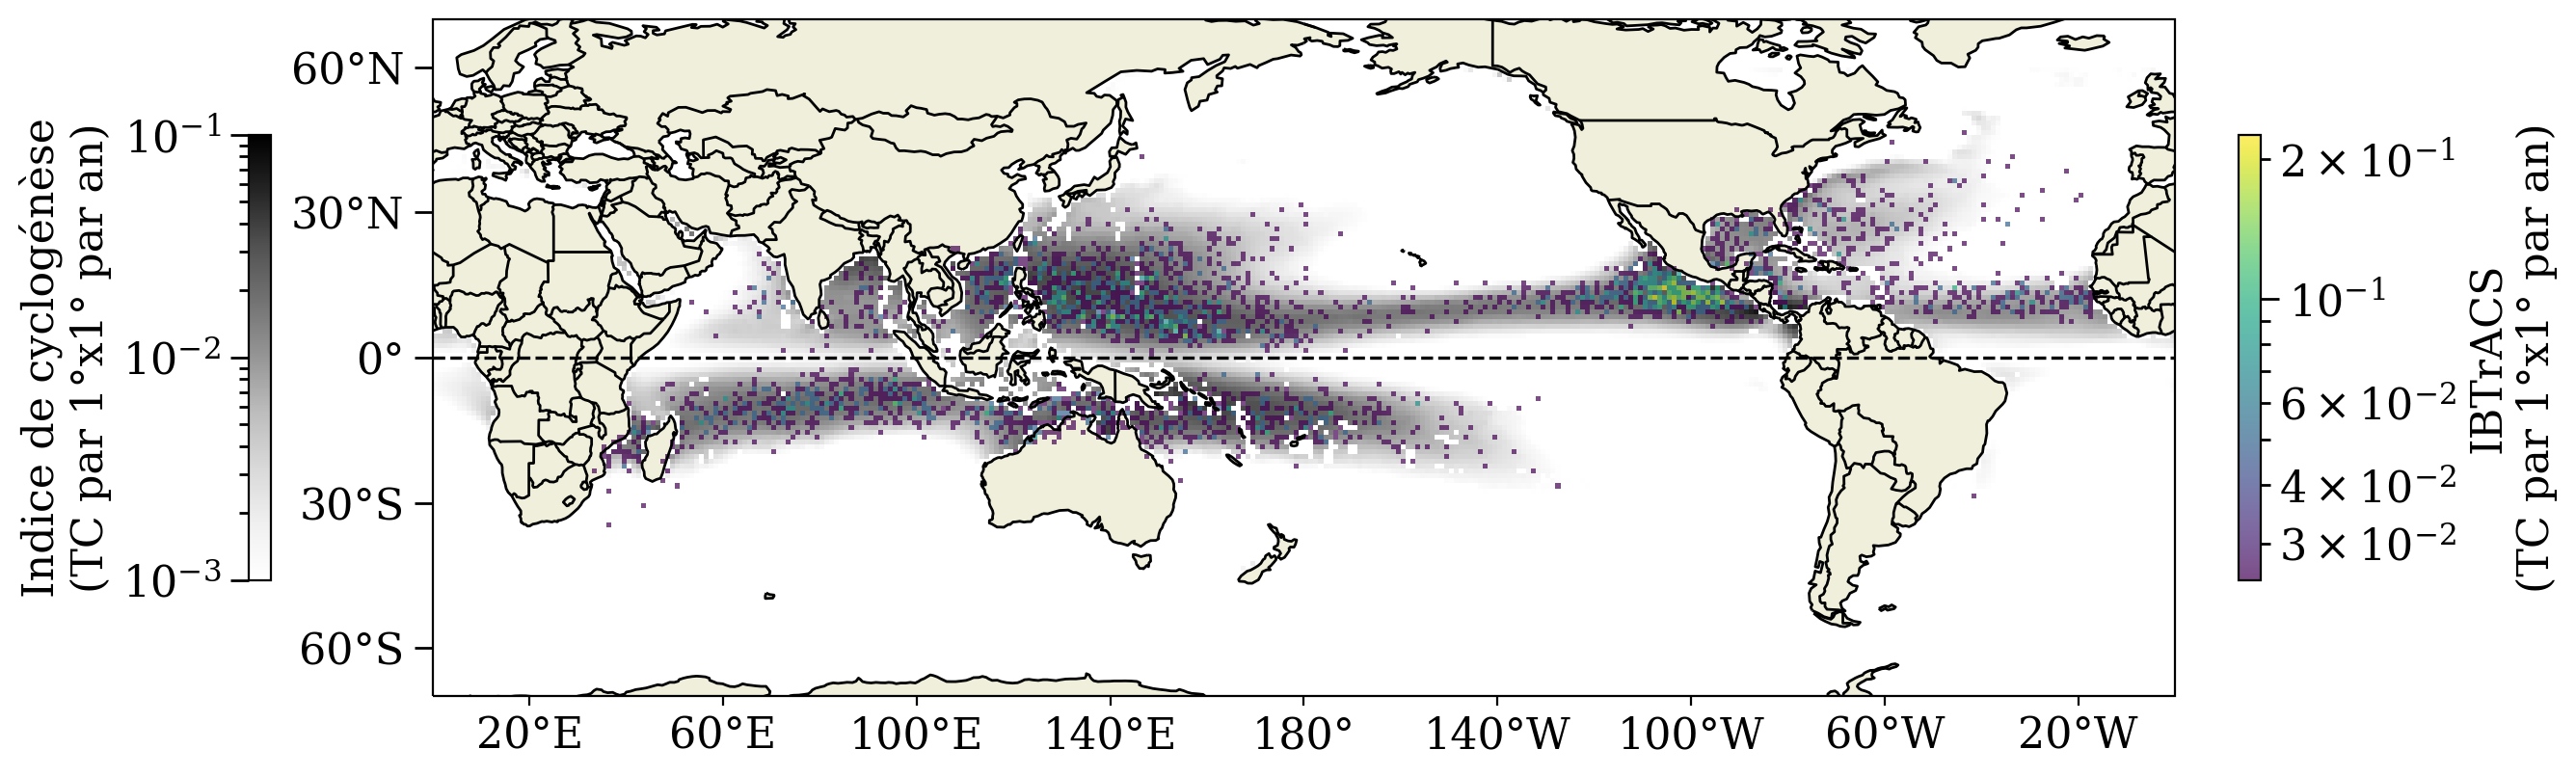
\includegraphics[width=\textwidth]{acgi_mean_IBTrACS.png}
    \caption{Moyenne temporelle de la moyenne du TCS, du GPI et CYGP évalués sur ERA5 à \ang{1} de résolution entre 1980 et 2020 (nuances de gris). Densité
    moyenne de cyclogénèses IBTrACS sur une grille de même résolution et sur la même période.}
    \label{fig:acgi_ibt}
\end{figure}

\subsubsection*{Distribution méridionale}

La \cref{fig:tcs_cygp_gpi_zonal} présente la distribution méridionale de l'activité pour les trois indices explicités dans la \cref{sec:tour_horizon_indices} et
évalués sur les moyennes mensuelles ERA5 entre \num{1981} et \num{2019}, comparée à celle d'IBTrACS sur la même période. 
%
\begin{figure}[htb]
    \centering
    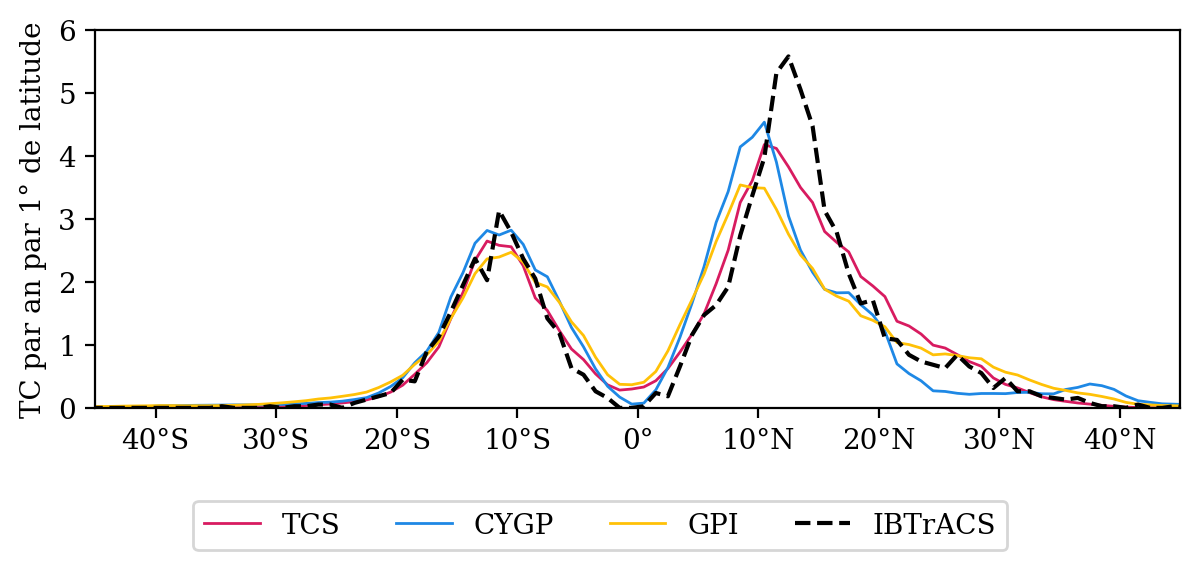
\includegraphics[width=0.8\textwidth]{tcs_cygp_gpi_ibt_zonal_sum_1981_2019.png}
    \caption{Intégrale zonale de la moyenne annuelle du TCS, CYGP et du GPI calculés sur les champs mensuels ERA5 interpolés sur une grille régulière de 1° de
    résolution horizonale, entre 1981 et 2019. Le tracé en tirets indique la distribution méridionale annuelle moyenne des premières observations des systèmes
    IBTrACS renseignés comme tempêtes tropicales ou subtropicales sur la même période et sur la même grille spatiale.}
    \label{fig:tcs_cygp_gpi_zonal}
\end{figure}
%
Comme indiqué par \textcite{menkes_comparison_2012}, qui évaluent ces trois mêmes indices (ainsi que le YGP) sur quatre réanalyses antérieures à ERA5, les trois
indices tendent à surévaluer l'activité cyclonique à proximité de l'équateur, aussi bien dans l'hémisphère nord que dans le sud. Sur ERA5, seul le CYGP atteint
quasiment 0 à l'équateur (\num{0.05} TC par an à exactement 0° par interpolation quadratique, les points de grille les plus proches étant \ang{0.5}S et
\ang{0.5}N), tandis que le TCS et le GPI y simulent respectivement \num{0.3} et \num{0.4} TC par an.

Dans l'hémisphère sud, les trois indices ainsi que les
observations sont en bon accord pour ce qui concerne l'amplitude de l'activité méridionale moyenne ainsi que sa position. Le maximum des observations est
atteint à la latitude \ang{11.5}S avec \num{3.13} TC par an. Le TCS, CYGP et le GPI quant à eux ont une latitude du maximum de respectivement \ang{12.5}S,
\ang{10.5}S et \ang{10.5}S. Les trois indices atteignent donc leur maximum aux latitudes directement voisines du maximum d'IBTrACS, de part et d'autre de
celle-ci, l'espacement étant de \ang{1}. Le CYGP simule le pic le plus fort et au plus proche des observations avec \num{2.9} TC par an à la latitude du
maximum, suivi dans l'ordre du TCS (\num{2.7} TC par an) et enfin du GPI (\num{2.5} TC par an). Notons toutefois que, lorsqu'intégré entre \ang{60}S et
l'équateur, le TCS produit l'activité la plus proche des observations, avec \num{26.8} TC par an contre \num{26.1} TC par an dans IBTrACS (voir aussi
\cref{tab:tcs_cygp_gpi}). Les deux autres indices surestiment également l'activité totale de cet hémisphère avec \num{31.9} TC par an pour le CYGP et \num{30.7}
TC par an pour le GPI. En effet, si les trois indices surévaluent l'activité à proximité de l'équateur, le CYGP et le GPI la surestiment également dans les
latitudes plus basses, là où le TCS suit fidèlement IBTrACS. Dans l'hémisphère sud, la cohérence entre les trois indices et les observations est améliorée par
rapport aux résultats obtenus par \textcite{menkes_comparison_2012}, notamment sur ERA-40, distante d'ERA5 de deux générations.

Dans l'hémisphère nord, les performances des trois indices sont nettement plus contrastées. Ni l'amplitude, ni la position du pic d'activité, ni l'étendue
méridionale des trois indices ne correspondent aux observations. Ils présentent tous un biais équatorial plus ou moins prononcé, avec une différence de \ang{4}
pour le GPI et de \ang{2} pour le TCS et le CYGP dans la latitude du maximum. Bien que le CYGP et le TCS partagent la même latitude du maximum, le biais
équatorial du CYGP est distinctement plus prononcé que pour le TCS, ce dernier présentant la meilleure ressemblance avec IBTrACS. Rappelons que les indices
simulent, par construction, \num{84.7} TC par an entre \ang{60}S et \ang{60}N. Par conséquent, si les indices surestiment l'activité dans l'hémisphère sud, cela
signifie mécaniquement qu'ils la sous-estiment dans le nord. La somme des biais dans les deux hémisphères est donc nulle. Il en résulte que le TCS présente là
aussi la meilleure activité totale intégrée entre \ang{0} et \ang{60}N avec un déficit de \num{0.7} TC par an. Le GPI arrive en seconde position avec un déficit
de \num{4.5} TC par an tandis que le CYGP présente un déficit plus conséquent de \num{5.7} TC par an. Le CYGP se distingue également par un regain d'activité
entre \ang{35}N et \ang{40}N, évalué à \num{1.3} TC par an sur cette bande. Ainsi, sur ERA5, les trois indices surestiment l'activité cyclonique annuelle
moyenne dans l'hémisphère sud, et la sous-estiment dans le nord. Le TCS présente toutefois la meilleure répartition de l'activité entre hémisphère, ainsi que la
meilleure distribution méridionale.

\subsubsection*{Climatologie mensuelle}

La \cref{fig:tcs_cygp_gpi_clim_mensuel} présente quant à elle la climatologie mensuelle pour les trois indices, évaluée selon le même mode opératoire que pour
la \cref{fig:tcs_cygp_gpi_zonal} ---~à cela près que l'intégration spatiale des indices est réalisée aussi bien en longitude qu'en latitude~--- pour IBTrACS et
pour les 6 bassins océaniques d'intérêt, les frontières de ces derniers étant tracées sur la \cref{fig:bassins_TC} du \cref{chap:chapitre_1}, ainsi que dans la
\cref{sec:papier_appendix_B} du \cref{chap:chapitre_2} \parencite[][documents supplémentaires]{dulac_assessing_2023}. Là encore, les trois indices se
distinguent les uns des autres par des cycles saisonniers aux propriétés variables, bien que tous soient capables de reproduire approximativement la
climatologie observée. 

\begin{figure}[tb]
    \centering
    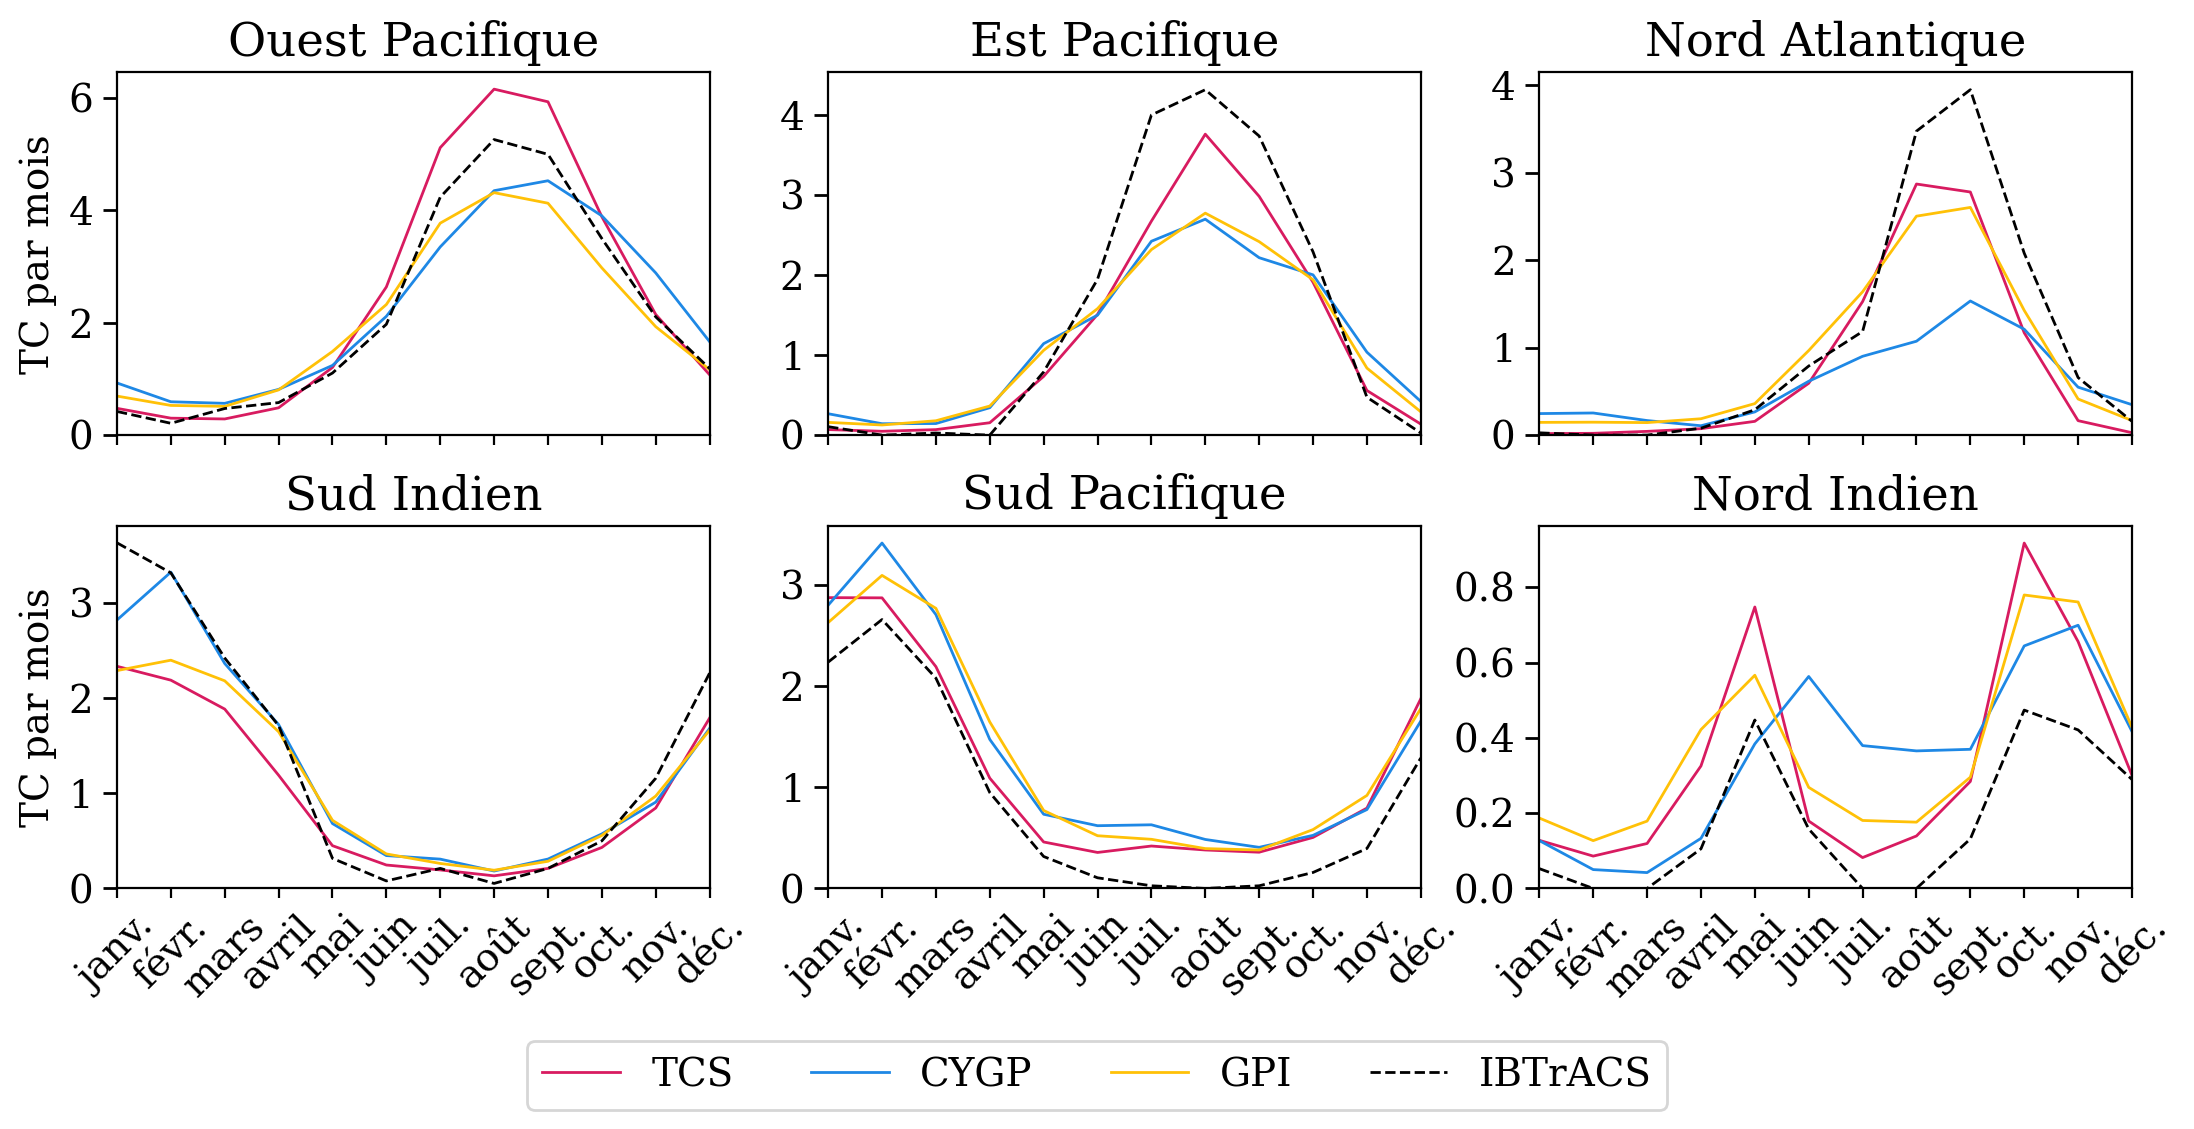
\includegraphics[width=\textwidth]{tcs_cygp_gpi_ibt_clim_mensuel.png}
    \caption{Cycle annuel de l'activité cyclonique inférée par les trois indices de cyclogénèses définis dans la \cref{sec:tour_horizon_indices} sur
    ERA5 entre 1981 et 2019. Le tracé en tirets noirs indique la climatologie mensuelle observée d'après IBTrACS sur la même période.}
    \label{fig:tcs_cygp_gpi_clim_mensuel}
\end{figure}

Les qualités désirables pour la climatologie mensuelle d'un indice de cyclogénèse à l'échelle régionale sont de pouvoir simuler : la bonne saisonnalité, c'est à
dire la bonne étendue temporelle, y compris en minimisant l'activité en dehors de la saison ; la bonne amplitude ; et naturellement le bon nombre de TC moyen
par an. Sur l'ensemble de ces aspects, aucun des trois indices n'apparaît comme clairement supérieur aux autres sur l'ensemble des six bassins d'activité. Les
trois indices capturent correctement la saison cyclonique dans l'ensemble des bassins, à l'exception du CYGP dans le Nord Indien où le pic de la première saison est
indiqué pour le mois de juin plutôt que mai pour les deux autres et dans les observations. Cette caractéristique du CYGP est également notée dans
\textcite{menkes_comparison_2012}, et ne saurait s'expliquer par l'utilisation des précipitations convectives, puisque le YGP présente le même attribut (mais
encore plus prononcé) et trouve par conséquent son origine dans la composante dynamique de l'indice. Le CYGP se démarque par ailleurs du TCS et du GPI à deux
autres reprises : dans le bassin Nord Atlantique où celui-ci sous-estime très fortement l'amplitude de l'activité (voir aussi \cref{tab:tcs_cygp_gpi}) ; et dans
le bassin Sud-Indien, où il est au contraire le seul à simuler un maximum réaliste au mois de février, bien que la tendance entre janvier et février soit
mauvaise. Le TCS se démarque une de fois de plus comme étant l'indice le plus apte à minimiser l'activité inférée en dehors de la saison cyclonique, bien
qu'elle ne soit tout de même pas négligeable entre juin et octobre dans le bassin SPac, simulant environ \num{0.5} TC par mois, ainsi que dans le NInd entre
juin et août. Par ailleurs, tous les indices surestiment l'activité dans ces deux bassins. Il est toutefois difficile de distinguer la contribution d'IBTrACS de
celle des indices dans ce constat dans la mesure où les observations dans ces bassins y sont moins fiables que dans les autres régions ; en particulier dans le
NInd, où elles sont quasi inexistantes jusqu'au début des années 2000. Les pic d'activités simulés par le TCS dans le WPac, EPac, NAtl et NInd sont
supérieurs à ceux du CYGP et du GPI. Dans le WPac, le TCS dépasse même les observations sur la période juillet~--~août~--~septembre. Dans les deux bassins de
l'hémisphère sud, l'activité inférée par le TCS est au contraire plus faible que pour les deux autres indices (ce qui pour le SPac aboutit à une meilleure
représentation de l'activité observée). Cela se comprend d'une part par le fait, montré dans la section précédente, que le CYGP et le GPI surestiment l'activité
dans l'hémisphère sud tandis qu'ils la sous-estiment dans le nord ---~le TCS étant beaucoup plus proche des observations dans les deux hémisphères~--- et
d'autre part, par la capacité du TCS à capturer plus finement la saison active, en débordant moins que les autres sur la saison creuse. Dans le nord, cela
creuse l'écart du TCS par rapport aux deux autres au cœur de la saison active, tandis qu'il est permis de penser que cette propriété tend au contraire à
compenser l'activité moindre dans le sud. Sans être exempt de tout défaut, le TCS réunit donc, dans l'ensemble, le plus de qualités désirables dans un indice de
cyclogénèse pour simuler la climatologie mensuelle à l'échelle régionale.
\subsection*{Fréquence annuelle et variabilité}

La première partie du \cref{tab:tcs_cygp_gpi} présente la fréquence annuelle moyenne TC dans les six bassins géographiques ainsi que pour chaque hémisphère et à
l'échelle globale. Notons en premier lieu que les trois indices produisent le bon ordre de grandeur de fréquence annuelle à toutes les échelles spatiales, avec
l'exception éventuelle de la sous-estimation du CYGP dans le NAtl, et des trois indices dans le bassin NInd, ce dernier pouvant être dû au manque
d'observations dans la région. Le TCS apparait comme l'indice simulant le nombre moyen annuel de TC le plus proche d'IBTrACS pour \num{5} des \num{8} échelles
spatiales considérées (l'échelle globale ne comptant pas, puisque la fréquence annuelle globale est imposée), à savoir dans le EPac, SPac, NInd et pour les deux
hémisphères. Dans le WPac et le SInd, le TCS est toutefois le plus éloigné de la réalité, et est le seul à produire un surplus dans le WPac, avec $+$\num{3.1}
TC par an par rapport à IBTrACS. Il occupe enfin la 2\ieme~place du classement dans le bassin NAtl, devant le CYGP. Le CYGP quant à lui se démarque dans le WPac
---~bien qu'il ait tendance à simuler une saison légèrement trop tardive, décalée d'environ 1 mois, c.f \cref{fig:tcs_cygp_gpi_clim_mensuel}~--- et dans le
SInd. Enfin, le GPI ne produit la fréquence annuelle la plus proche d'IBTrACS que pour le bassin NAtl, avec cependant un déficit de \num{2.2} TC par an. Dans le
sous-ensemble d'IBTrACS utilisé ici, le ratio de la fréquence annuelle moyenne entre les deux hémisphères est de \num{2.16}. Sans surprise, le TCS en est le
plus proche, avec une différence inférieure à \num{0.01}. Le GPI arrive en seconde position avec \num{1.76} et enfin le CYGP avec \num{1.66}.

\begin{table}[tb]
    \centering
    \caption{Caractéristiques du TCS, du CYGP et du GPI calculés sur ERA5 entre 1981 et 2019 comparé à IBTrACS, par bassin océanique, pour chaque hémisphère
    ainsi qu'à l'échelle globale. Les valeurs en gras renseignent pour chaque colonne l'indice se rapprochant le plus des observations.}
    \begin{tabular}{lrrrrrrrrr}
        \toprule\toprule
        & WPac & EPac & NAtl & SInd & SPac & NInd & NH & SH & Global\\
        \midrule
        \multicolumn{10}{r}{\textbf{Fréquence (TC par an)}}\\
        IBTrACS & \num{26} & \num{17.7} & \num{12.7} & \num{15.9} & \num{10.2} & \num{2} & \num{58.5} & \num{26.1} & \num{84.7}\\
        \midrule
        TCS & \num{29.7} & \textbf{\num{14.6}} & \num{9.4} & \num{11.9} & \textbf{\num{14.2}} & \textbf{\num{4}} & \textbf{\num{57.8}} & \textbf{\num{26.9}} &
        \num{84.7}\\
        CYGP & \textbf{\num{26.9}} & \num{14.3} & \num{7.3} & \textbf{\num{15.2}} & \num{16.2} & \num{4.2} & \num{52.8} & \num{31.9} & \num{84.7}\\
        GPI & \num{29.7} & \num{14} & \textbf{\num{10.7}} & \num{13.5} & \num{16} & \num{4.4} & \num{54} & \num{30.7} & \num{84.7}\\
        \midrule
        \multicolumn{10}{r}{\textbf{Corrélation interannuelle avec IBTrACS}}\\
        TCS & \num{0.03} & \textbf{\num{0.7}} & \num{0.71} & \num{-0.13} & \num{0.35} & --- & \num{0.31} & \num{-0.07} & $<$ \num{0.01} \\
        CYGP & \textbf{\num{0.46}} & \num{0.62} & \num{0.7} & \textbf{\num{-0.13}} & \textbf{\num{0.57}} & --- & \num{0.27} & \textbf{\num{0.05}} & \num{0.01}\\
        GPI & \num{0.06} & \num{0.64} & \textbf{\num{0.79}} & \num{-0.3} & \num{0.39} & --- & \textbf{\num{0.43}} & \num{-0.09} & \textbf{\num{0.17}}\\
        \bottomrule
    \end{tabular}
    \label{tab:tcs_cygp_gpi}
\end{table}

La seconde partie du \cref{tab:tcs_cygp_gpi} présente la corrélation interannuelle des trois indices de cyclogénèses avec IBTrACS pour les mêmes échelles
spatiales. Notons que la variabilité interannuelle est évaluée pour les saisons cycloniques de \num{1981} à \num{2019}, si bien que son calcul fait intervenir
dans l'hémisphère sud les valeurs de l'indice depuis juillet 1980 jusqu'à juin 2019. Cela est valable aussi pour la variabilité à l'échelle globale, évaluée
comme la somme des séries temporelles calculées indépendamment l'une de l'autre sur les deux hémisphères. Précisons également que la variabilité interannuelle
dans IBTrACS pour le bassin NInd est largement composée de \num{0} jusqu'au début des années 2000, raison pour laquelle les corrélations sont omises dans cette
colonne. Là encore, aucun indice ne se distingue clairement des deux autres à toutes les échelles. La capacité des trois indices à produire une variabilité
interannuelle corrélée aux observations est très variable selon les régions du monde et selon les indices. En effet, les trois indices indiquent une corrélation
négative dans le SInd, jusqu'à \num{-0.3} pour le GPI. Dans le WPac, le TCS et le GPI ne présentent aucune corrélation, tandis que le CYGP indique un
coefficient, certes faible mais sensiblement meilleur que pour les deux autres, de \num{0.46}. À l'inverse, dans les bassins EPac et NAtl, les trois indices
indiquent une variabilité interannuelle en phase avec IBTrACS. En effet dans l'EPac, le TCS indique une corrélation de \num{0.7}, suivi du GPI avec \num{0.64}
et enfin du CYGP à \num{0.62}, tandis que le GPI dans le NAtl atteint la plus haute corrélation de \num{0.79} ---~le TCS et le CYGP présentant des performances
honorables d'environ \num{0.7} chacun. Le CYGP se distingue aussi dans le SPac avec une corrélation relativement faible de \num{0.57}, mais meilleure que les
deux autres indices puisque celles-ci valent \num{0.39} et \num{0.35} pour le GPI et le TCS, respectivement. À plus grande échelle, la variabilité interannuelle
des indices dans l'hémisphère nord est plus proche que dans le sud, avec dans le premier cas, entre \num{0.27} pour le CYGP et \num{0.43} pour le GPI, tandis
que dans l'hémisphère sud les trois indices indiquent une corrélation quasi-nulle. À l'échelle globale, seul le GPI indique une très maigre corrélation de
\num{0.17}, les deux autres indices ne présentant une fois de plus aucun lien avec les observations. Séparer le bassin SInd en deux sous-bassins s'avère
bénéfique pour la corrélation interannuelle des trois indices. Spécifiquement, on définit le bassin Sud Ouest Indien (SIndW) entre \ang{20}E et \ang{90}E de
longitude, puis le bassin Sud Est Indien (SIndE), correspondant au bassin australien, entre \ang{90} et \ang{135}E. La limite méridionale demeure inchangée,
entre \ang{0} et \ang{60}S. Ce découpage est plus proche du découpage pratiqué pour la surveillance opérationnelle, comme expliqué dans la
\cref{sec:bassins_saisons} du \cref{chap:chapitre_1}. Dans ce contexte, le TCS présente une corrélation de \num{0.21} et \num{0.22} pour le SIndW et le SIndE
respectivement ; \num{0.37} et \num{0.16} pour le CYGP ; \num{0.27} et \num{0.12} pour le GPI. Par conséquent, et pour la suite des travaux présentés dans ce
document, nous distinguerons toujours les régions SIndW et SIndE.

\begin{figure}[tb]
    \centering
    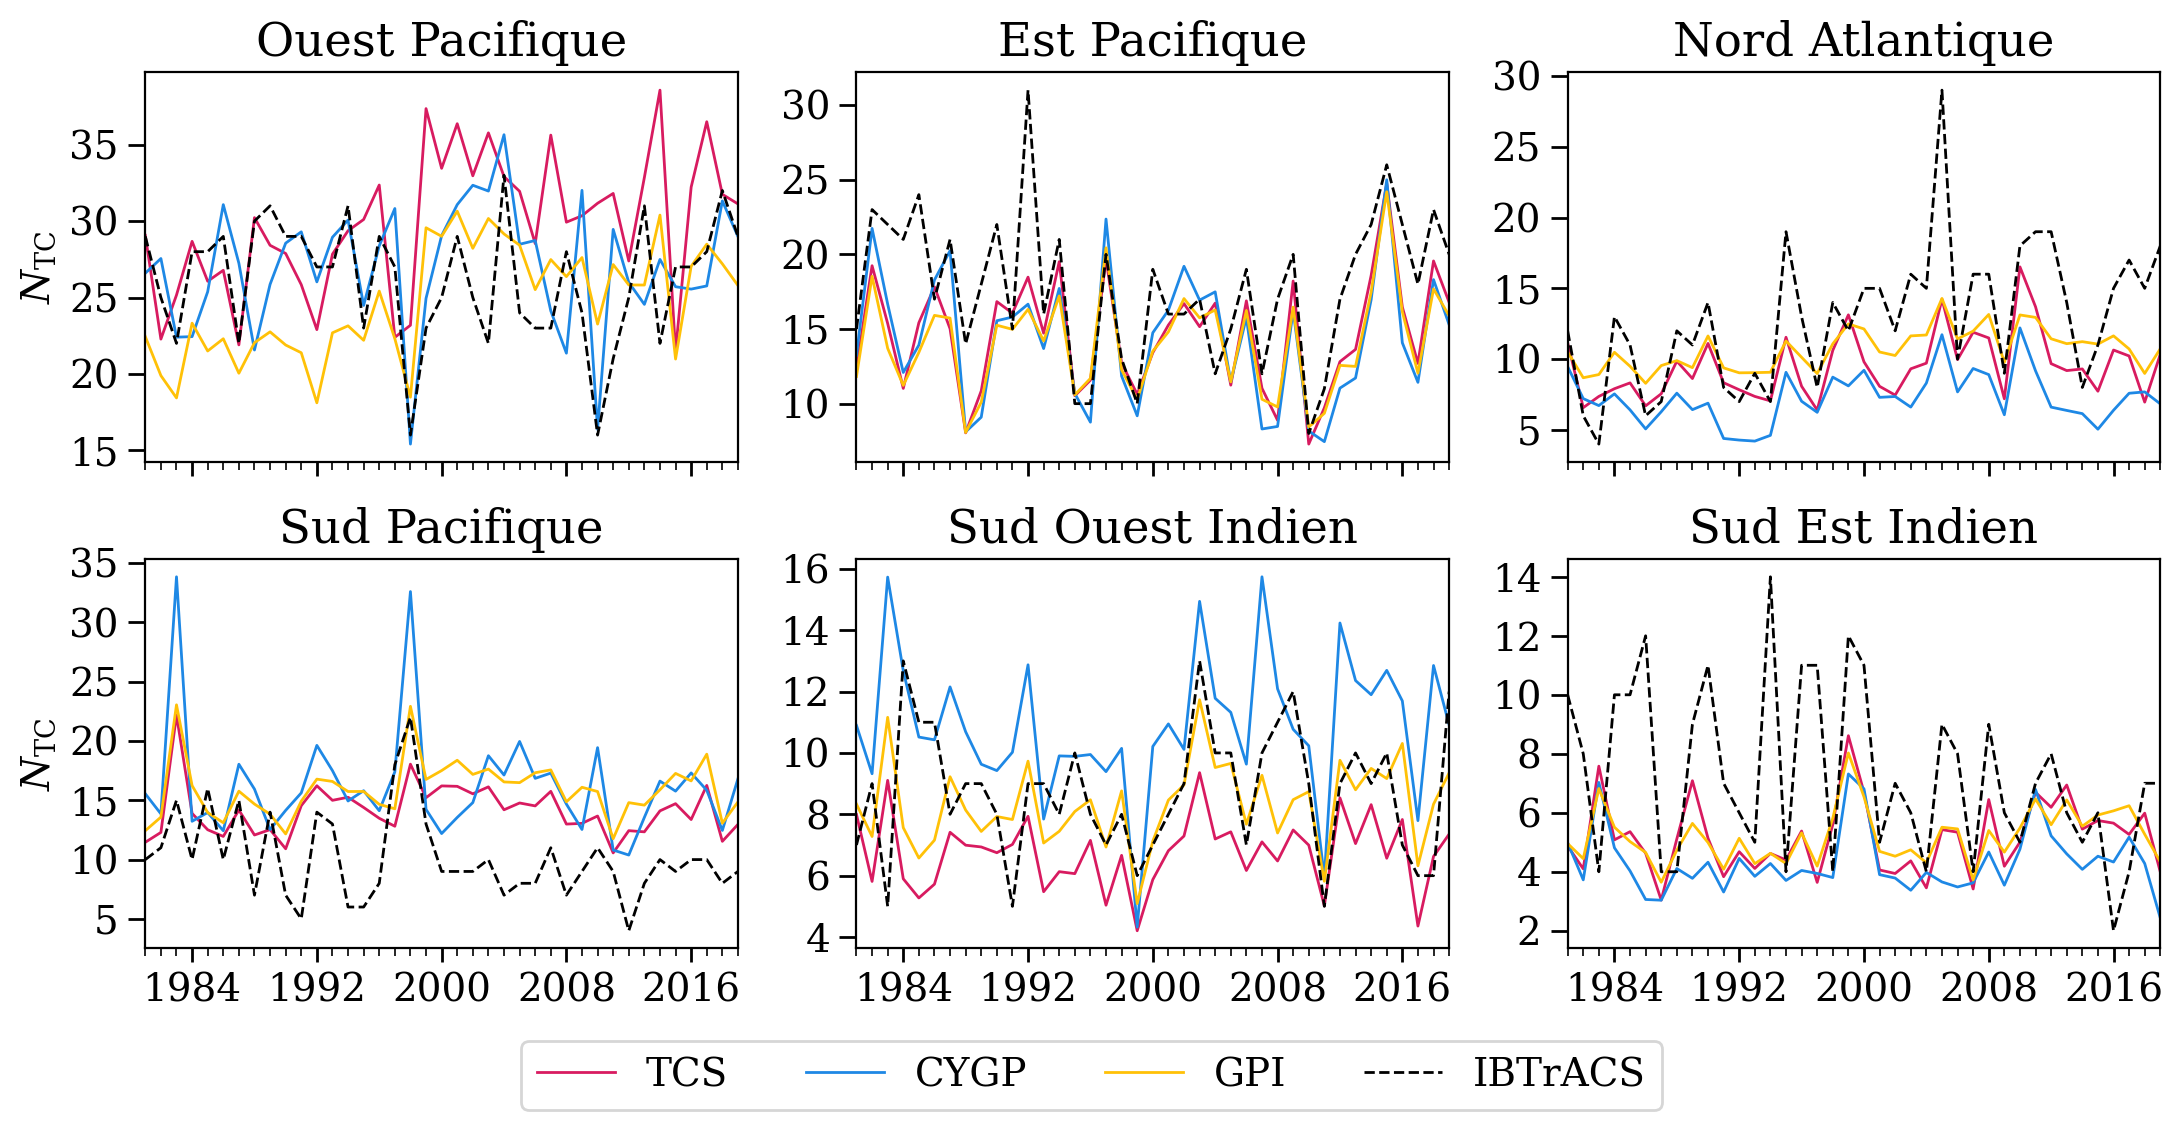
\includegraphics[width=\textwidth]{tcs_cygp_gpi_interannual.png}
    \caption{Variabilité interannuelle entre 1981 et 2019 inférée pour le TCS, le CYGP et le GPI, comparé à IBTrACS.}
    \label{fig:tcs_cygp_gpi_variabilite}
\end{figure}

Enfin, il est important de préciser qu'une bonne corrélation ne présage en rien de la capacité d'un indice à simuler une amplitude réaliste de sa variabilité
interannuelle. La \cref{fig:tcs_cygp_gpi_variabilite} présente les séries temporelles de variabilité interannuelles entre les saisons cycloniques \num{1981} et
\num{2019} dont sont issues les corrélations du \cref{tab:tcs_cygp_gpi}. Dans le bassin NAtl, où la corrélation interannuelle est supérieure à \num{0.7} pour
les indices, l'amplitude de la variabilité inférée est moindre par rapport aux observations. Cela est particulièrement vrai pour le GPI, présentant un
écart-type de \num{1.4} TC contre \num{4.8} TC dans IBTrACS. Le TCS présente une amplitude plus forte que le GPI, mais cette dernière reste toutefois faible,
avec un écart-type de \num{2.3}, soit une dispersion plus de deux fois petite que la dispersion observée. Certains sursauts observés sont cependant capturés par
les trois indices. C'est notamment le cas de l'année \num{1995} et \num{2005}. Dans le Sud Pacifique et Sud Est Indien, le constat est similaire, avec une forte
sous-estimation de l'amplitude à l'exception de certains pics comme pour la saison \num{1998} dans le SPac. Le sursaut d'activité simulé par le CYGP est par
ailleurs anormalement élevé, par rapport aux observations ainsi qu'aux deux autres indices, dépassant \num{32} TC. Cette valeur n'est dépassée qu'en \num{1983}
avec près de \num{34} TC, le GPI et le TCS étant quant à eux en accord sur une valeur de \num{23} TC et \num{22.2} respectivement. Si ces pics notés dans les
trois indices correspondent à un maximum local dans les observations également, la saison ne se démarque toutefois pas des autres saisons. En revanche, le
bassin EPac présente un accord remarquable entre la variabilité simulée et la variabilité observée, avec pour seules exceptions l'année \num{1992}, pic majeur
dans IBTrACS avec \num{31} systèmes, là où les trois indices indiquent entre \num{18.5} TC pour le TCS et \num{16.3} TC pour le GPI. La variabilité inférée par
les indices est, de manière générale, nettement moins proche d'IBTrACS avant l'année \num{1993}, puisque le seul désaccord au delà de cette année \num{2000}.
Notons en effet que la corrélation interannuelle pour le bassin EPac pris à partir de \num{1993} est augmentée d'au moins \num{0.1} par rapport aux valeurs
renseignées dans le \cref{tab:tcs_cygp_gpi}, atteignant \num{0.81} pour le TCS. Dans l'EPac, SInd (ouest et est), les trois indices présentent des variabilités
extrêmement semblables, mis à part les différences dans la fréquence moyenne dans le SIndW. Les différences sont plus marquées dans le WPac, en particulier
entre le GPI et les deux autres. Le CYGP apparait parfois en opposition du signal indiqué par le TCS et le GPI comme par exemple pour les années \num{1988} et
\num{2007}.

\subsection{Limitations des indices de cyclogénèses}

Les indices de cyclogénèses couramment utilisés dans la littérature et présentés ici mettent en évidence une grande capacité à simuler la répartition spatiale et
temporelle de l'activité cyclonique moyenne. Spatialement, les indices présentent un accord important dans l'hémisphère sud, aussi bien entre eux qu'avec les
observations. Dans l'hémisphère nord, la répartition méridionale est plus contrastée et tous les indices présentent un biais équatorial plus ou moins
conséquent. Le TCS se distingue comme le plus apte à simuler cette distribution, ainsi que la répartition de la fréquence annuelle globale entre les deux
hémisphères. De plus, le TCS et le GPI sont tous deux capables de simuler un cycle annuel réaliste dans les 6 bassins océaniques majeurs, tandis que le CYGP
montre des faiblesses dans le NInd et dans le NAtl, où l'activité est fortement sous-estimée, ainsi que dans une mesure bien moindre dans le WPac où avec un
retard d'un mois. Le TCS présente la qualité de discriminer plus finement la saison active de la saison creuse, résultant en une activité cyclonique hors saison
réduite par rapport aux deux autres indices. La fréquence annuelle à l'échelle régionale, ou plus exactement sa proximité avec la fréquence observée, est
variable selon les bassins, mais les trois indices apparaissent comme capables de simuler le bon ordre de grandeur pour chacun des bassins (à l'exception NInd,
probablement en raison du manque de fiabilité des observations dans cette région). Le TCS se démarque toutefois comme produisant la fréquence annuelle la plus
réaliste dans 5 des 8 échelles spatiales considérées.

À l'échelle interannuelle, les performances des trois indices apparaissent comme nettement moins bonnes. À l'exception de certains bassins, tels que le EPac et
le NAtl, la corrélation interannuelle demeure très faible, voire inexistante. De plus, les indices peinent souvent à simuler une amplitude réaliste de cette
variabilité. Ces caractéristiques ne concernent pas seulement la réanalyse ERA5 et sont connues de longue date
\parencite{watterson_seasonal_1995,camargo_tropical_2007,tippett_poisson_2011,menkes_comparison_2012,wang_dynamic_2020,cavicchia_tropical_2023a}. La question de
la variabilité interannuelle inférée par les indices apparaît ici comme un élément central pour espérer comprendre la divergence dans les projections futures
entre les approches directes et indirectes. En effet, outre la question de la stationnarité des relations entre l'environnement de grande échelle et l'activité
cyclonique en climat futur, on peut aussi se demander quelle confiance accorder dans la tendance du changement de l'activité cyclonique inférée par un indice de
cyclogénèse dans des scénários climatiques donnés pour la fin du siècle si ce dernier n'est pas en mesure de renseigner le bon changement d'une année sur
l'autre dans le climat présent, climat sur lequel l'indice est pourtant construit.

Les indices de cyclogénèse étant principalement conçus pour reproduire la climatologie observée de l'activité cyclonique, il n'est pas nécessairement surprenant
que ces derniers peinent à simuler la variabilité de l'activité d'une année sur l'autre. De plus, rappelons que ces indices sont établis sur la base des
climatologies saisonnières (à l'origine) ou mensuelle des champs de grande échelle, et à des résolutions grossières, de \ang{2.8} pour le CYGP
\parencite{royer_gcm_1998} et \ang{2.5} pour le TCS \parencite{tippett_poisson_2011}, l'applicabilité des indices aux modèles de climat à basses résolutions
étant en effet un de leurs atouts principaux (voir \cref{sec:intro_indices}). Or, si dans l'ensemble la capacité des indices à simuler l'activité cyclonique
moyenne est plutôt robuste aux changements de résolution, surtout comparé à la mesure par détection et suivi objectif \parencite[][voir aussi
\cref{fig:GP_resolution}]{camargo_tropical_2007}, il est tout de même à noter que les indices appliqués à des résolutions plus fines produisent plus de TC. Ce
point est également corroboré par \textcite{mcdonald_tropical_2005} qui notent une meilleure cohérence entre l'activité mesurée par approche directe et celle
inférée par les indices (spécifiquement avec le YGP et CYGP) pour les résolutions les plus hautes, amenant alors \textcite{camargo_tropical_2007} à spéculer
qu'une résolution accrue pourrait s'accompagner d'une réponse plus réaliste dans les variations interannuelles du nombre de TC inféré par les indices. Si les
indices analysés ici et calculés sur des champs ERA5 à \ang{1} de résolution ne présentent pas d'amélioration sensible en ce sens, on peut toutefois se demander
si un indice construit sur des champs à plus haute résolution (et pas seulement appliqué dessus) verrait une amélioration de sa variabilité interannuelle
inférée. De la même manière, les travaux de \textcite{bruyere_investigating_2012,waters_largescale_2012} suggèrent qu'il pourrait être pertinent pour la
représentation de la variabilité interannuelle des indices de chercher à les définir à des échelles régionales, ainsi que d'y intégrer de la variabilité à plus
haute fréquence, plutôt que de les construire sur la climatologie mensuelle globale.

Ce sont ces questions qui sont explorées dans la suite de ce chapitre ; l'enjeu est ici de chercher à améliorer la variabilité interannuelle des indices pour avoir une plus grande confiance dans leurs projections climatiques. Dans un premier temps, nous utiliserons la méthodologie de construction d'un indice de
cyclogénèse de \textcite{tippett_poisson_2011}, c'est à dire une régression de Poisson, pour définir et comparer des variantes du TCS à différentes résolutions
spatiales et temporelles. Nous chercherons en particulier comme ces facteurs influent sur les coefficients de la régression, et comment ceux-ci influencent en
retour la variabilité interannuelle. Étant construit comme une régression statistique entre l'environnement de grande échelle et l'activité observée, cet indice
possède en effet l'avantage d'être reproductible, contrairement aux deux autres qui sont dérivés de manière semi empiriques. Dans une autre partie, nous
construirons un indice de cyclogénèse régional, ou plus exactement un indice pseudo-global défini comme une aggrégation d'indices régionaux ---~également
construits par régression de Poisson~--- caractérisés par des coefficients propres à chaque région, pour là aussi voir comment la variabilité interannuelle s'en
retrouve affectée.

%Dans un premier temps, nous nous interrogerons sur l'apport de l'utilisation de champs
%mensuels plutôt que saisonniers dans la capacité de l'indice à simuler la climatologie saisonnière spatiale et temporelle, à l'aide des trois indices définis
%dans la \cref{sec:tour_horizon_indices}, à savoir le TCS, le CYGP et le GPI. Ensuite, nous étudierons l'apport de la résolution spatiale et temporelle,
%séparémment, pour la représentation de la variaiblité interannuelle. Spécifiquement, nous utiliserons des indices établis selon le mode opératoire de
%\textcite{tippett_poisson_2011}, à savoir par régression de Poisson, de façon à déterminer comment ces facteurs influent sur les coefficients de la régression,
%et comment ceux-ci influencent en retour la variabilité interannuelle. Enfin, nous regarderons si un indice construit comme une agrégation spatiale de
%régressions faites à l'échelle du bassin améliore ou non la variabilité interannuelle.

%--------------------------------------
%\section{Climatologie saisonnière spatiale et temporelle}

\section{Apport de la résolution spatiale et temporelle}\label{sec:apport_res_temporel_spatial}

On s'intéresse dans cette section à l'impact de la résolution spatiale et temporelle sur la variabilité interannuelle d'un indice de cyclogénèse défini comme
une régression de Poisson, selon \textcite{tippett_poisson_2011}. Pour cela, nous réalisons la régression entre l'activité observée, issue de la base de données
IBTrACS, et les prédicteurs de grande échelle constituant le TCS à deux résolutions différentes, puis en utilisant des moyennes mensuelles et la climatologie
mensuelle de ces champs, issus de la réanalyse ERA5. Cela revient donc à recalculer les coefficients $b$ issus de \textcite{tippett_poisson_2011} et donnés
dans la \cref{sec:modelisation_stat}, qui furent déterminés avec la climatologie mensuelle des prédicteurs des réanalyses NCEP
\parencite{kalnay_ncep_1996,kistler_ncep_2001} et ERA-40 \parencite{uppala_era40_2005} sur une grille de \ang{2.5} de résolution horizontale, et ce dans le but
d'estimer d'une part l'impact de la résolution spatiale et temporelle sur les coefficients de la régression, mais aussi l'impact des coefficients sur la
variabilité interannuelle.

\subsection{Données et méthodes}\label{sec:apport_res_methodes}

\subsubsection*{Régression de Poisson}\label{sec:regression_poisson}

Une régression de Poisson est un modèle statistique dans lequel la variable de réponse représente des données de comptage, ou de fréquence, sous la forme
d'entiers positifs (ou nuls). Une variable aléatoire $Y$ possède une distribution de Poisson de paramètre $\mu$ si la probabilité pour la variable $Y$
de prendre la valeur $k$ vaut :
%
\begin{equation*}
    P(Y = k) = \frac{e^{-\mu} \, \mu^k}{k!} \quad (k=0, 1, 2, \ldots) 
\end{equation*}
%
Où $\mu$ est égal à l'espérance de la variable aléatoire $Y$, ainsi qu'à sa variance. Dans ce cas, le logarithme de l'espérance de la variable $Y$ est relié
à la matrice $\mathbf{x}$ des prédicteurs, de taille $m \times n^\prime$, où $n^\prime = n + 1$ ---~composée de $n$ variables thermiques ou dynamiques, ainsi que
d'une constante unitaire, chacun avec $m$ réalisations~--- par le vecteur colonne $\mathbf{b}^{\mathrm{T}}$ des coefficients $b$, de taille $n^\prime$, de la
façon suivante :
%
\begin{gather*}
    \log \mathbb{E} \left( Y \mid \mathbf{x} \right ) = \mathbf{b}^{\mathrm{T}} \mathbf{x} \\
    %\Leftrightarrow \quad \quad \mathbb{E} \left ( Y \mid \mathbf{x} \right ) &= e^{\mathbf{b}^{\mathrm{T}} \mathbf{x}}
    \Leftrightarrow \quad \mu = e^{\mathbf{b}^{\mathrm{T}} \mathbf{x}}
\end{gather*}
%
Dans le cas qui nous intéresse, la variable $Y$ représente un nombre de TC par unité de temps et par unité de surface, si bien qu'on introduit le terme
d'\textquote{exposition} de l'unité (\textit{exposure} en anglais), $\cos \phi$, où $\phi$ représente la latitude, comme proxy de la surface d'une maille. On a
alors :
%
\begin{equation}
    \begin{gathered}\label{eq:poisson_reg}
        \log \left( \frac{\mathbb{E} \left( Y \mid \mathbf{x}\right )}{\cos \phi} \right) = \mathbf{b}^{\mathrm{T}} \mathbf{x} \\
        %\Leftrightarrow \quad\quad \log \mathbb{E} \left( Y \mid \mathbf{x} \right) &= \mathbf{b}^{\mathrm{T}} \mathbf{x} + \log (\cos \phi)
        \Leftrightarrow \quad \log \mu = \mathbf{b}^{\mathrm{T}} \mathbf{x} + \log (\cos \phi)
    \end{gathered}
\end{equation}

%
Ce qui revient également à ajouter $\log (\cos \phi)$ comme prédicteur avec un coefficient de pondération fixé à 1.

Pour définir un indice de cyclogénèse par régression de Poisson, la variable $Y$ est composée du nombre de cyclogénèses, issu soit d'observations (donc
d'IBTrACS, si la régression est évaluée contre ERA5) soit des trajectoires détectées par un schéma de détection objectif. Dans tous les cas, on considère que
les cyclogénèses sont données par les positions des premières échéances de chaque trajectoire. Les cyclogénèses sont comptabilisées sous la forme d'histogrammes
sur une grille spatiale identique à celle des variables de grande échelle, lesquels étant au besoin interpolés à la résolution désirée. Ces histogrammes spatiaux des
cyclogénèses sont ensuite agrégés temporellement selon le pas de temps désiré : mensuel ou climatologiques, là encore de la même manière que les prédicteurs.
Les cyclogénèses, servant de prédictant, forment alors un tenseur du deuxième ordre, qui se voit ensuite ramené en un vecteur unidimensionnel de taille $m =
N_{\mathrm{lat}} \times N_{\mathrm{lon}} \times N_{\mathrm{temps}}$, définissant le vecteur des observations\footnote{Le terme \textquote{observation}, dans ce
contexte, est à comprendre au sens statistique du terme, et ne présage en rien de si les cyclogénèses sont réellement des observations historiques ou bien
issues d'un schéma de détection appliqué aux sorties d'un modèle de climat ou d'une réanalyse atmosphérique.} $Y$. Le procédé est répété pour chacune des $n$
variables de grande échelle qui sont ensuite concaténées entre elles, ainsi qu'avec le vecteur unitaire de même taille pour former la matrice $\mathbf{x}$.
C'est à ce vecteur unitaire qu'est associé le coefficient $b_0$ dans la formulation du TCS. L'ajustement de la relation \ref{eq:poisson_reg} sur les données
$Y$, composées de $m$ observations $Y_i$, et sur $\mathbf{x}$, composée de $m$ réalisations $\mathbf{x}_i$ (c'est à dire les lignes de la matrice $\mathbf{x}$,
représentant un point de grille quelconque à une date quelconque) fournies en entrée consiste alors à identifier les coefficients de pondération de $\mathbf{b}
= (b_0, b_1, b_2, \, \ldots \, , b_n)$ qui maximisent la fonction de log-vraisemblance $\ell (\mathbf{b})$, donnée ci-dessous à titre de référence, et qui est
définie comme la somme des logarithmes de la vraisemblance de chacune des observations.
%
\begin{equation*}
    \begin{cases}
        \ell(\mathbf{b}) = \sum_{i = 1}^{m} Y_i \log \mu_i - \mu_i - \log(Y_i !) \\
        \log \mu_i = \mathbf{b}^{\mathrm{T}} \mathbf{x}_i + \log ( \cos \phi )
    \end{cases}
\end{equation*}

Une régression de Poisson présuppose que la variable aléatoire qui est modélisée est régie par une loi de Poisson, et donc que sa moyenne soit égale à sa
variance. Il arrive toutefois que cette hypothèse ne soit pas vérifiée. Pour s'en prémunir, on utilise ici l'estimation de la covariance de
\textcite{mackinnon_heteroskedasticityconsistent_1985}, possédant la propriété d'être robuste à l'hétéroscédasticité. L'usage de cette méthode se traduit par un
intervalle de confiance des coefficients $b$ ajusté, mais n'affecte pas les valeurs des coefficients eux-mêmes. C'est donc une méthode analogue à celle dite
\textquote{quasi-Poisson} utilisée par \textcite{tippett_poisson_2011}. Notons enfin que, comme le souligne \textcite{tippett_poisson_2011}, les coefficients de
la régression s'interprètent comme des sensibilités. En particulier, un changement unitaire d'une des variables de grande échelle $x_j$, $j = (1, 2, \ldots, n)$
se traduit par la modification de la fréquence attendue de cyclogénèses d'un facteur $e^{b_j}$. Pour des faibles valeurs de $b$, on a $e^{b_j} \approx 1 + b_j$,
soit une modification attendue de $(100 \cdot b_j)$~\%. Par exemple, le coefficient $b_H = \num{0.05}$ du TCS indique une réponse attendue de la fréquence de
cyclogénèses d'approximativement $+$\prct{5} pour un changement de 1 unité de l'humidité relative à \hPa{600}.

\subsubsection*{Construction des indices}\label{sec:construction_indices}

On s'intéresse ici à la construction d'indices composés des mêmes prédicteurs que le TCS, définis dans la \cref{sec:modelisation_stat}. Rappelons seulement
brièvement que l'indice est composé de la vorticité absolue bornée $\eta = \min(\zeta, \num{3.7})$, du cisaillement vertical entre \hPa{850} et \hPa{200}
$V_{\mathrm{shear}}$, de l'humidité relative à \hPa{600} $H$, et de la SST relative, définie comme l'écart entre la SST et la SST moyennée entre \ang{20}S et
\ang{20}N. Ces prédicteurs sont issus de la réanalyse ERA5 entre \num{1980} et \num{2019}, et sont pris à l'échelle globale, entre \ang{60}S et \ang{60}N. On
utilise comme prédictant la base de données IBTrACS, version 4 \parencite{knapp_international_2010}. Spécifiquement, on conserve les positions des premières
échéances des systèmes renseignés par leurs métadonnées comme étant des tempêtes tropicales ou subtropicales, à un moment donné de leur cycle de vie, de la même
manière que dans la \cref{sec:proprietes_indices}.

Quatre indices sont construits par régression de Poisson, en utilisant des champs à \ang{1.0} et \ang{2.5}, ainsi qu'en appliquant la régression donnée par la
relation \ref{eq:poisson_reg} sur les champs mensuels ERA5 (un pas de temps par mois et par an) ou bien sur leurs valeurs climatologiques (un pas de temps par mois obtenu par moyenne sur les années). Le premier, nommé C25 (comme \textquote{climatologie}, et
\ang{2.5}) utilise les moyennes climatologiques des champs de grande échelle ainsi que des cyclogénèses IBTrACS sur une grille de \ang{2.5}. D'un point de vue
méthodologique, seules la réanalyse utilisée ainsi que la période temporelle considérée distingue les coefficients $b$ de C25 de ceux du TCS, ces derniers étant
en effet également issus de valeurs climatologiques à cette même résolution. C25 joue alors pour ainsi dire le rôle de groupe témoin, car il est attendu que ses
coefficients soient les plus proches possibles de ceux du TCS. Notons que pour cet indice, on a $m = N_{\mathrm{lat}} \times N_{\mathrm{lon}} \times N_{\mathrm{temps}} = \num{48} \times \num{144} \times \num{12}$. Toutefois,
l'emploi d'un masque terre-mer approprié réduit la taille des vecteurs, car les points de terre masqués sont ignorés. La taille effective, $m_{\mathrm{eff}}$,
vaut ici \num{52128} (au lieu de \num{82944}). Le second indice, nommé C10, est quant à lui établi toujours sur les moyennes climatologiques, mais avec une
résolution de \ang{1.0} ($m_{\mathrm{eff}} = \num{327876}$). Le troisième, M25 est construit sur les moyennes mensuelles ($N_{\mathrm{temps}} = \num{480}$) à
\ang{2.5}, et donc avec $m_{\mathrm{eff}} = \num{2085120}$. Enfin le dernier, nommé M10, correspond par conséquent, selon la nomenclature utilisée jusqu'à
maintenant, à une régression faite sur les moyennes mensuelles ERA5 à une résolution de \ang{1.0}, conduisant à la plus grande matrice $\mathbf{x}$,
caractérisée par $m_{\mathrm{eff}} = \num{13115040}$. Notons qu'au pas de temps mensuel, la taille de la matrice $\mathbf{x}$ est le facteur limitant la
résolution spatiale. C'est là une des raisons faisant qu'ERA5 n'est pas utilisée à sa pleine résolution de \ang{0.25}, puisque la régression sur un nombre de
réalisations $m_{\mathrm{eff}}$ plus grand nécessiterait des ressources de calcul supplémentaires.

Ces quatre nouveaux indices ainsi que le TCS sont ensuite évalués sur les champs ERA5 au pas de temps mensuel et à \ang{1} de résolution, et sur la même période,
indépendant de la résolution spatiale et de l'agrégation temporelle utilisée pour calculer la régression. On ne se préoccupe pas de répartir l'ensemble des
données entre un jeu d'apprentissage et un jeu d'évaluation dans la mesure où le surapprentissage ne constitue ici pas un risque, mais au contraire une
propriété désirable.

\subsection{Résultats}\label{sec:apport_resultat}

Le \cref{tab:fit_spatial_temporel} présente les coefficients $b$ des multiples régressions qui sont réalisées. Les coefficients du TCS sont rappelés et indiqués
dans le tableau à titre de référence. Les coefficients sont donnés avec quatre décimales, telles que données par la régression car celles-ci ne varient pas lorsque les régressions sont répétées.
Les erreurs standards issues de la régression pour chacun des coefficients et des indices sont également indiquées, comparés à celles indiquées dans
\textcite{tippett_poisson_2011} pour le TCS. Tous les coefficients estimés ici apparaissent comme statistiquement significatifs à \prct{95}, au sens où, à ce
niveau de confiance, il n'y a pas d'incertitude sur le signe des coefficients.

\begin{table}[htpb]
    \centering
    \caption{Estimation des coefficients des régressions de Poisson établies entre les quatre variables de grande échelle du TCS, issues d'ERA5, et l'activité
    observée issue d'IBTrACS entre 1980 et 2019. La colonne \textquote{Temporelle} correspond à la valeur $N_{\mathrm{temps}}$.}
    \label{tab:fit_spatial_temporel}

    \resizebox{\textwidth}{!}{
    \begin{tabular}{crrrrrrrr}
       \toprule\toprule 
       \textbf{Indice} & \multicolumn{5}{c}{\textbf{Coefficients}} & \multicolumn{3}{c}{\textbf{Résolution}}\\
       \midrule
              & $b_0$ & $b_{\eta}$ & $b_{V_{\mathrm{shear}}}$ & $b_H$ & $b_T$ & Spatiale     & Temporelle & $m_{\mathrm{eff}}$ \\
       \midrule
              & \multicolumn{5}{l}{Estimations} & & & \\
       C25    & \num{-11.1927} & \num{1.0538} & \num{-0.1051} & \num{0.0653}  & \num{0.4396} & \ang{2.5}  & 12  & \num{52128} \\
       C10    & \num{-13.1570} & \num{1.0702} & \num{-0.1034} & \num{0.0655}  & \num{0.4584} & \ang{1.0}  & 12  & \num{327876} \\ 
       M25    & \num{-13.0987} & \num{1.3757} & \num{-0.0976} & \num{0.0726}  & \num{0.3967} & \ang{2.5}  & 480 & \num{2085120} \\
       M10    & \num{-15.0496} & \num{1.3968} & \num{-0.0960} & \num{0.0718}  & \num{0.4142} & \ang{1.0}  & 480 & \num{13115040} \\
       \midrule
       TCS    & \num{-5.8}     & \num{1.03}   & \num{-0.15}   & \num{0.05}    & \num{0.56}   & \ang{2.5}  & 12  & --- \\
       \midrule
              &\multicolumn{5}{l}{Erreur standard} & & &\\
        C25 & \num{0.194} & \num{0.029} & \num{0.005} & \num{0.002} & \num{0.019} & & &\\
        C10 & \num{0.164} & \num{0.026} & \num{0.004} & \num{0.002} & \num{0.017} & & &\\
        M25 & \num{0.161} & \num{0.031} & \num{0.004} & \num{0.002} & \num{0.015} & & &\\
        M10 & \num{0.162} & \num{0.032} & \num{0.004} & \num{0.002} & \num{0.015} & & &\\
        \midrule
        TCS & \num{0.19} & \num{0.026} & \num{0.01} & \num{0.003} & \num{0.021} & & &\\
       \bottomrule
    \end{tabular}
    }
\end{table}

Le premier constat concerne le terme d'ordonnée à l'origine $b_0$, largement différent du TCS pour les quatre régressions. Celui-ci est cependant difficile à
interpréter dans le contexte de la modélisation de la fréquence d'occurrence de cyclogénèses. Il est supposé que ce terme soit lié à l'état moyen des
prédicteurs, si bien que l'écart entre les régressions faites ici et le TCS pour le terme $b_0$ serait principalement la conséquence de l'utlisation d'une
réanalyse différente, ainsi que d'une période temporelle différente. L'indice C25 présente les coefficients les plus proches du TCS, à l'exception, marginale,
du prédicteur de SST, noté $T$. En effet, le $b_{\mathrm{T}}$ de C10 est très légèrement plus proche de celui du TCS que ne l'est celui de C25. Les coefficients
du C25 montrent tout de même des écarts avec ceux du TCS, notamment pour les termes de cisaillement vertical et de SST relative. Spécifiquement,
$b_{V_{\mathrm{shear}}}$ vaut environ \num{-0.10} pour C25 contre respectivement \num{-0.15} pour le TCS, tandis que $b_T$ est réduit de \num{0.56} pour le TCS
à environ \num{0.44} pour C25. Cela signifie donc d'une part que le cisaillement vertical apparaît comme moins défavorable à la cyclogénèse dans C25 que dans
le TCS, et d'autre part que la fréquence d'occurrence des cyclones tropicaux est moins sensible à la SST relative pour C25 que dans le TCS. Comme pour le terme
d'ordonnée à l'origine, il est là aussi possible que ces différences proviennent de la réanalyse utilisée, mais on note toutefois une certaine sensibilité des
coefficients de C25 à la période temporelle utilisée. La régression C25 faite sur la période \num{1980}~--~\num{2000} produit en effet des coefficients se
rapprochant davantage de ceux du TCS, à savoir un $b_T$ réhaussé (\sim~\num{0.47}) et un $b_{V_{\mathrm{shear}}}$ diminué (\sim~\num{-0.11}), tandis que ceux
obtenus sur la période \num{2000}~--~\num{2019} présentent au contraire une valeur $b_T$ plus faible (\sim~\num{0.42}), et un $b_{V_{\mathrm{shear}}}$ plus
grand (\sim~\num{-0.09}). En tout état de cause, la proximité entre les paramètres de C25 et ceux du TCS, relativement aux trois autres régressions, valide la
reproduction de l'indice de \textcite{tippett_poisson_2011} et de la méthodologie associée, ce qui par extension, tend également à valider les coefficients
obtenus pour C10, M25 et M10, moyennant l'effet sus-mentionné de la période considérée.

L'effet de la résolution sur les coefficients $b$, en comparant C25 avec C10, et M25 avec M10, apparaît mince. Les coefficients présentent des changements
faibles, de l'ordre de \num{10}$^{\num{-2}}$, ou inférieur. $b_{\eta}$ est augmenté d'environ \num{0.02} pour l'indice climatologique comme l'indice mensuel.
L'ordre de grandeur du changement sur $b_{V_{\mathrm{shear}}}$ est d'environ \num{1e-3}. $b_H$ est stable pour l'indice climatologique, et présente une très
faible baisse pour dans M10 par rapport à M25, d'environ \num{1e-3}, tandis que $b_T$ augmente d'environ \num{2e-2}. L'ajout de variabilité temporelle dans la régression,
en utilisant les champs au pas de temps mensuels plutôt que les moyennes climatologiques, produit un effet plus conséquent sur les coefficients de la
régression. Le changement apporté à $b_{V_{\mathrm{shear}}}$ est d'un ordre de grandeur plus grand que le changement dû au passage à la résolution plus fine,
avec environ une augmentation de \num{10}$^{\num{-2}}$, pour l'indice à \ang{2.5} comme celui à \ang{1} de résolution. La sensibilité à l'humidité relative est
légèrement revue à la hausse lorsque sur les indices M, de l'ordre de \num{5e-3}, là aussi, indépendamment de la résolution. $b_T$ est diminué de manière un peu
plus importante, d'environ \num{4e-2}. L'impact le plus net se trouve cependant dans la vorticité. Celui-ci passe d'une moyenne de \num{1.062} entre C25 et C10,
à une moyenne de \num{1.3863} pour M25 et M10, soit une différence de $+$\num{0.3243}, autrement dit une augmentation de \prct{30.5} du coefficient $b_{\eta}$
par rapport au TCS.

\subsubsection{Répartition géographique}\label{sec:repartition_geographique}

L'effet du passage de \ang{2.5} à \ang{1} pour les régressions climatologiques et mensuelles se détermine en comparant C25 avec C10, et M25 and M10. Les deux
différences, $\mathrm{C25} - \mathrm{C10}$ et $\mathrm{M25} - \mathrm{M10}$ étant quasiment identiques, on décrit ici l'effet général du passage à une
résolution plus fine pour un indice construit selon la méthologie de \textcite{tippett_poisson_2011} comme la moyenne des deux différences. Le même constat est
fait pour l'emploi de champs mensuels dans la régression plutôt que des moyennes climatologiques, si bien que nous considérons la moyenne de $(\mathrm{M10} -
\mathrm{C10})$ et de $(\mathrm{M25} - \mathrm{C25})$. Les moyennes annuelles pour ces deux quantités sont présentées sur la \cref{fig:impact_spatial_temporel},
avec l'encadré (a) pour l'effet du passage à une résolution plus fine, et l'encadré (b) pour l'emploi de champs mensuels.

\begin{figure}[tb]
    \centering
    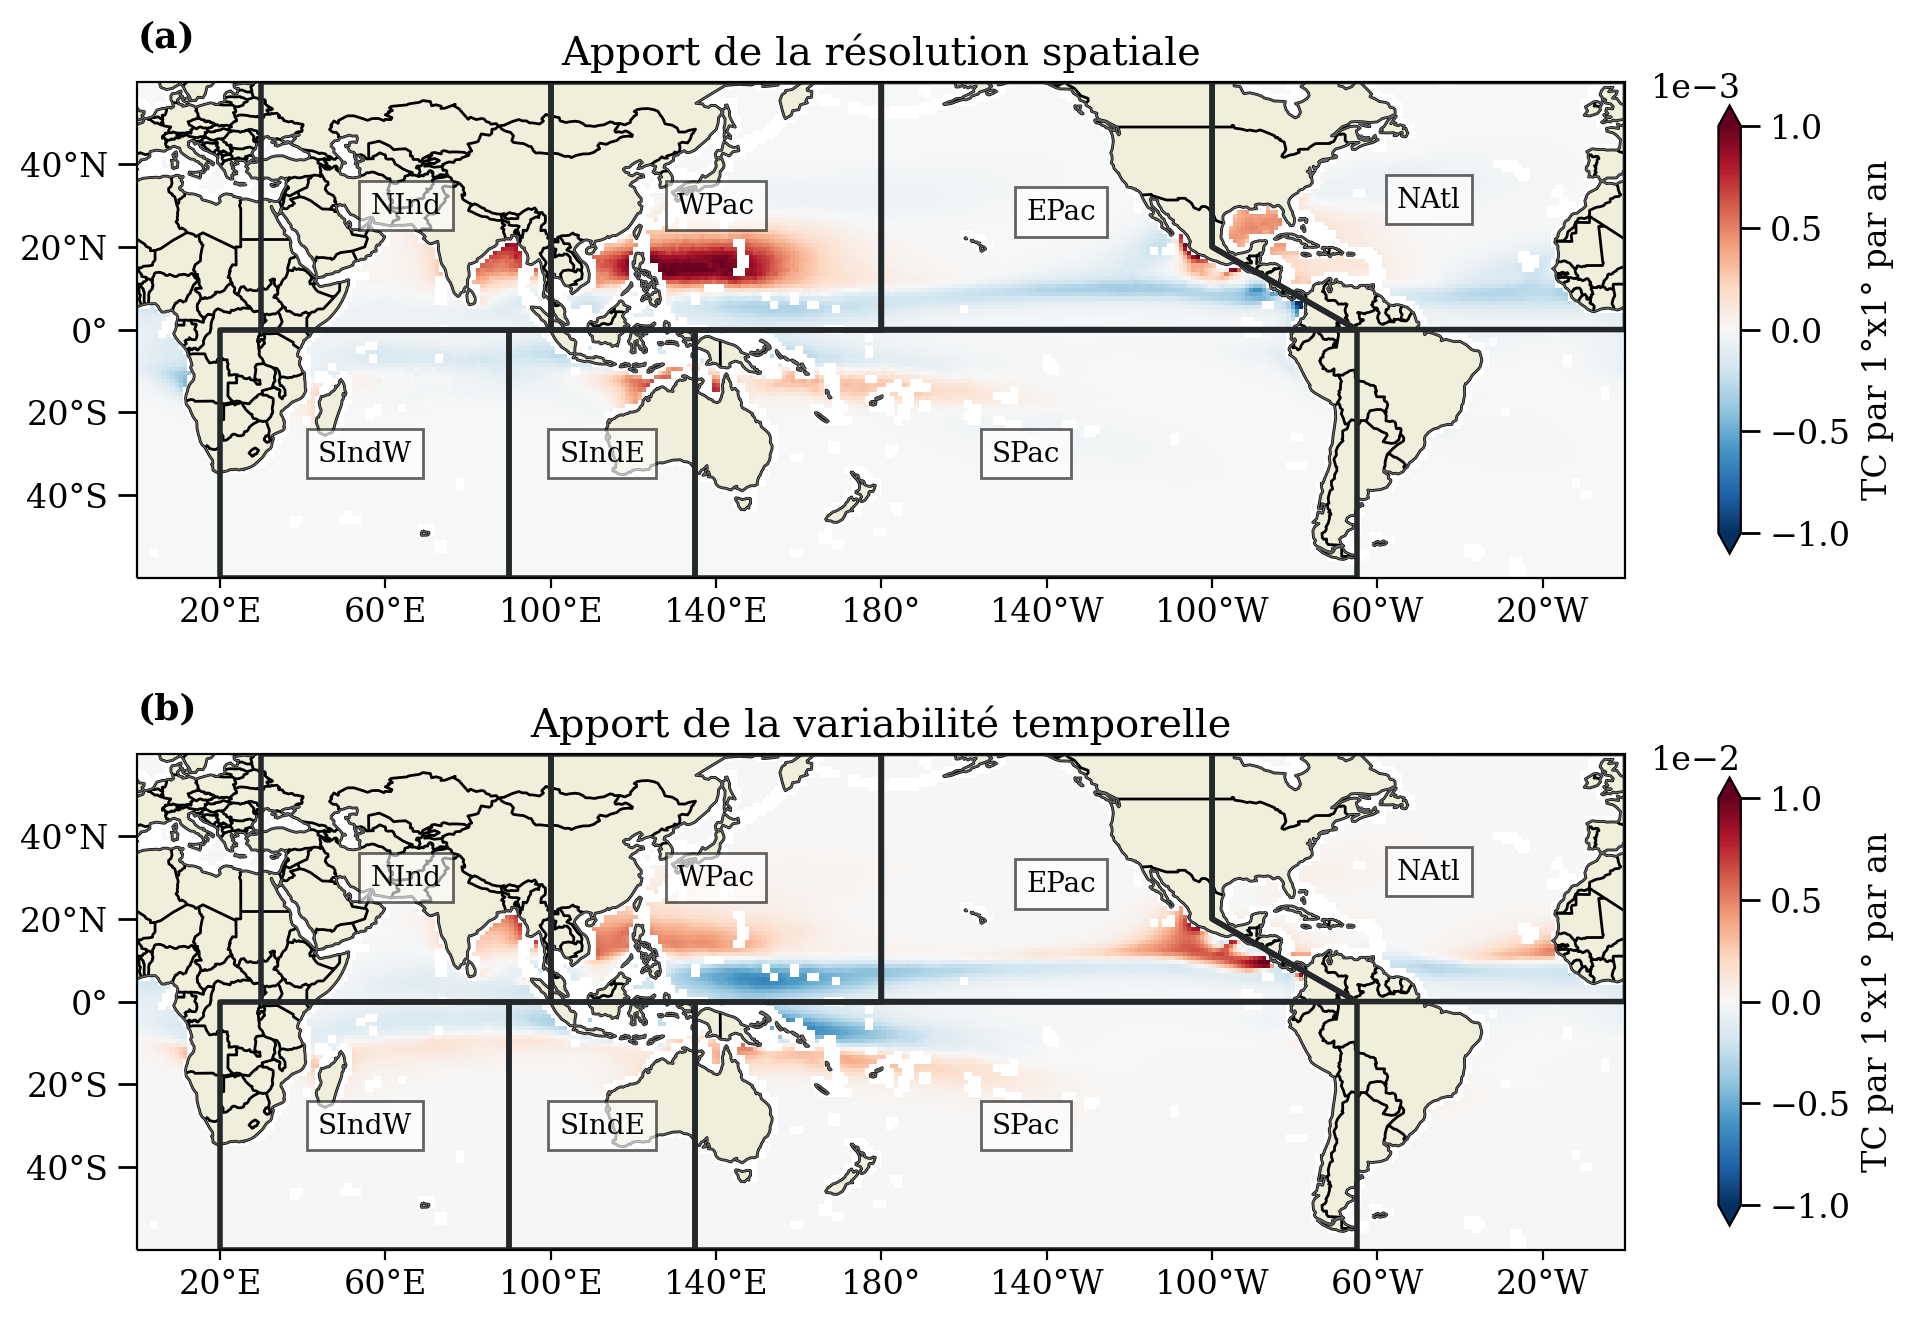
\includegraphics[width=\textwidth]{yearmean_spatial_temporel.png}
    \caption{Moyenne annuelle de (a) l'effet du passage de \ang{2.5} à \ang{1} de résolution, et (b) de l'effet de l'emploi de moyennes mensuelles plutôt que
    climatologiques pour les régressions décrites dans la \cref{sec:construction_indices}. Ces cartes sont construites avec la moyenne de (C10 $-$ C25) et de
    (M10 $-$ M25) pour (a), et avec la moyenne de (M10 $-$ C10) et de (M25 $-$ C25) pour (b). Les bassins géographiques usuels et leurs limites sont listés.}
    \label{fig:impact_spatial_temporel}
\end{figure}

Notons tout d'abord que si l'effet de la résolution spatiale accrue et celui de l'emploi des moyennes mensuelles partagent des similarités, l'effet des champs
mensuels dans la régression est un ordre de grandeur plus grand que l'effet de la résolution spatiale. Dans les deux cas, l'apport d'information spatiale plus
fine et de variabilité temporelle tend à décaler l'activité cyclonique plus loin de l'équateur, avec des spécificités selon les régions. Dans l'encadré (a),
l'activité, pour le bassin NAtl, l'activité est accrue dans le golf du Mexique (\textit{Gulf of Mexico}, GoM), au détriment de la zone de développement
principale (\textit{Main Development Region}, MDR, entre \ang{10}N et \ang{20}N et entre \ang{20}W et \ang{60}W.). Dans l'encadré (b) pour ce même bassin, le
GoM ne présente pas de variation importante, et l'effet de l'ajout de variabilité temporelle sur la MDR est contrasté, avec une baisse du côté de l'équateur
mais une augmentation la partie nord-est de la MDR. Dans les deux cas, l'intégrale sur le bassin est essentiellement \num{0}. Dans le EPac, l'effet de la
résolution spatiale accrue est en opposition avec l'effet de la variabilité mensuelle, notamment le long des côtes du Mexique. Les intégrales sont de signe
opposés, avec \num{-0.16} TC par an sur le panneau (a), et $+$\num{0.50} TC par an. On imagine alors que M10, combinant les deux effets, s'accompagne d'une très
légère hausse de la fréquence annuelle moyenne dans ce bassin. Dans le bassin WPac, les contributions sont inversées. En effet, si les deux panneaux indiquent
une hausse de l'acitivité autour de \ang{10}, en mer de Chine méridionale, et une diminution dans la région équatoriale, pour (a) l'augmentation l'emporte, avec
$+$\num{0.28} TC par an, tandis que pour (b) la diminution équatoriale est plus importante, avec \num{-0.12} TC par an. Dans le NInd, l'augmentation de
l'activité concerne principalement le golf du Bengale, la mer d'Arabie ne voyant elle que peu de changement, avec peut-être une très légère augmentation pour la
panneau (a). Les intégrales se compensent avec respectivement $+$\num{0.04} et \num{0.04} TC par an pour (a) et (b). Dans le SIndW, l'augmentation est plus
prononcée dans le canal du Mozambique, mais le panneau (b) laisse voir une augmentation au niveau de la bande de longitude à \ang{10}S, augmentation relative
absente du panneau (a). Le SIndE montre dans le (a) une augmentation relative prononcée au niveau des côtes au nord-ouest de l'Australie. Dans le SPac, l'effet
est comparable entre les deux panneaux, avec la même structure que partout ailleurs, c'est à dire un décalage de l'activité plus loin de la région équatoriale.
Précisons que par construction, les intégrales des deux champs moyens à l'échelle globale sont nulles.

\begin{figure}[htb]
    \centering
    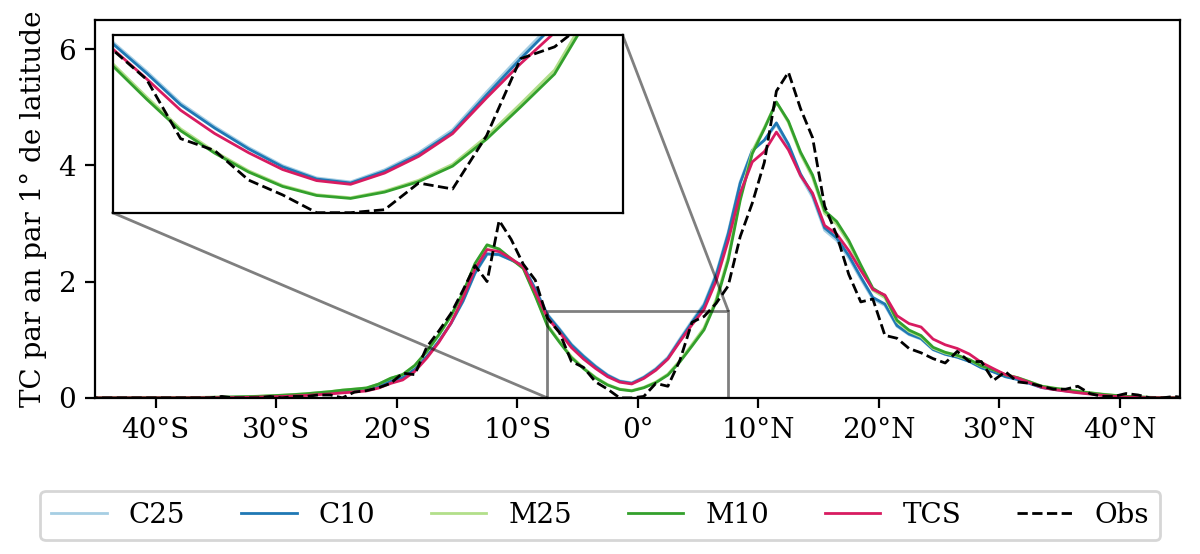
\includegraphics[width=0.8\textwidth]{C25_C10_M25_M10_TCS_IBTrACS_zonal.png}
    \caption{Comme pour la \cref{fig:tcs_cygp_gpi_zonal}, avec C25, C10, M25, M10 et le TCS, comparé à IBTrACS, ici noté \textquote{Obs}. Les paires de même
    aggrégation temporelle, c'est à dire C25 avec C10, et M25 avec M10 sont superposées. L'encadré en haut à gauche montre un grossissement entre \ang{7.5}S et
    \ang{7.5}N, et entre 0 et \num{1.5} TC par an.}
    \label{fig:my_fit_meridional}
\end{figure}

La \cref{fig:my_fit_meridional} présente la distribution méridionale des quatre indices nouvellement construits, ainsi que pour le TCS et IBTrACS, faite selon
les mêmes modalités que pour la \cref{fig:tcs_cygp_gpi_zonal}. La \cref{fig:my_fit_meridional} confirme ce que la \cref{fig:impact_spatial_temporel} laissait
entrevoir, à savoir une nette amélioration du biais équatorial pour les indices dont la régression est basée sur les moyennes mensuelles plutôt que
climatologiques. Le tracé de C10 est superposé à C25, indiquant que la résolution accrue ne suffit pas à modifier la distribution méridionale moyenne, en dépit
du signal en ce sens de l'encadré (a) de la \cref{fig:impact_spatial_temporel}. Les tracés pour M10 et M25 sont également superposés, et tous deux bénéficient
de l'amélioration. Rappelons que l'effet de l'ajout de variabilité temporelle dans la régression est d'un ordre de grandeur plus grand que celui de la
résolution spatiale plus fine, comme en attestent les échelles de couleur des encadrés (a) et (b) de la \cref{fig:impact_spatial_temporel}. Étant donnés les
coefficients des régressions du \cref{tab:fit_spatial_temporel}, il semblerait que la sensibilité accrue à la vorticité absolue bornée $\eta$ pour les indices
M10 et M25, résultant de l'ajout de variabilité temporelle dans la régression, soit à l'origine de la réduction du biais équatorial.

\subsubsection{Variabilité interannuelle}\label{sec:variabilite_5_indices}

Comme pour la \cref{fig:tcs_cygp_gpi_variabilite}, la variabilité interannuelle est calculée pour les saisons cycloniques et non pas pour les années
calendaires. Cela signifie que pour les bassins de l'hémisphère sud, à savoir le SPac, SIndW et SIndE, les indices et les observations sont, pour la saison $n$,
intégrées entre juillet de l'année calendaire $n-1$ et juin de l'année calendaire $n$. La \cref{fig:variabilite_basin_5_indices} présente la variabilité
interannuelle entre les saisons \num{1981} et \num{2019}, pour C25, C10, M25 et M10, ainsi que pour le TCS de \textcite{tippett_poisson_2011}, et IBTrACS (noté
\textquote{Obs} sur la \cref{fig:variabilite_basin_5_indices}). La colonne de droite sur la figure présente, pour chaque bassin, la matrice de corrélation entre
les 6 jeux de données.

\begin{figure}[p]
    \centering
    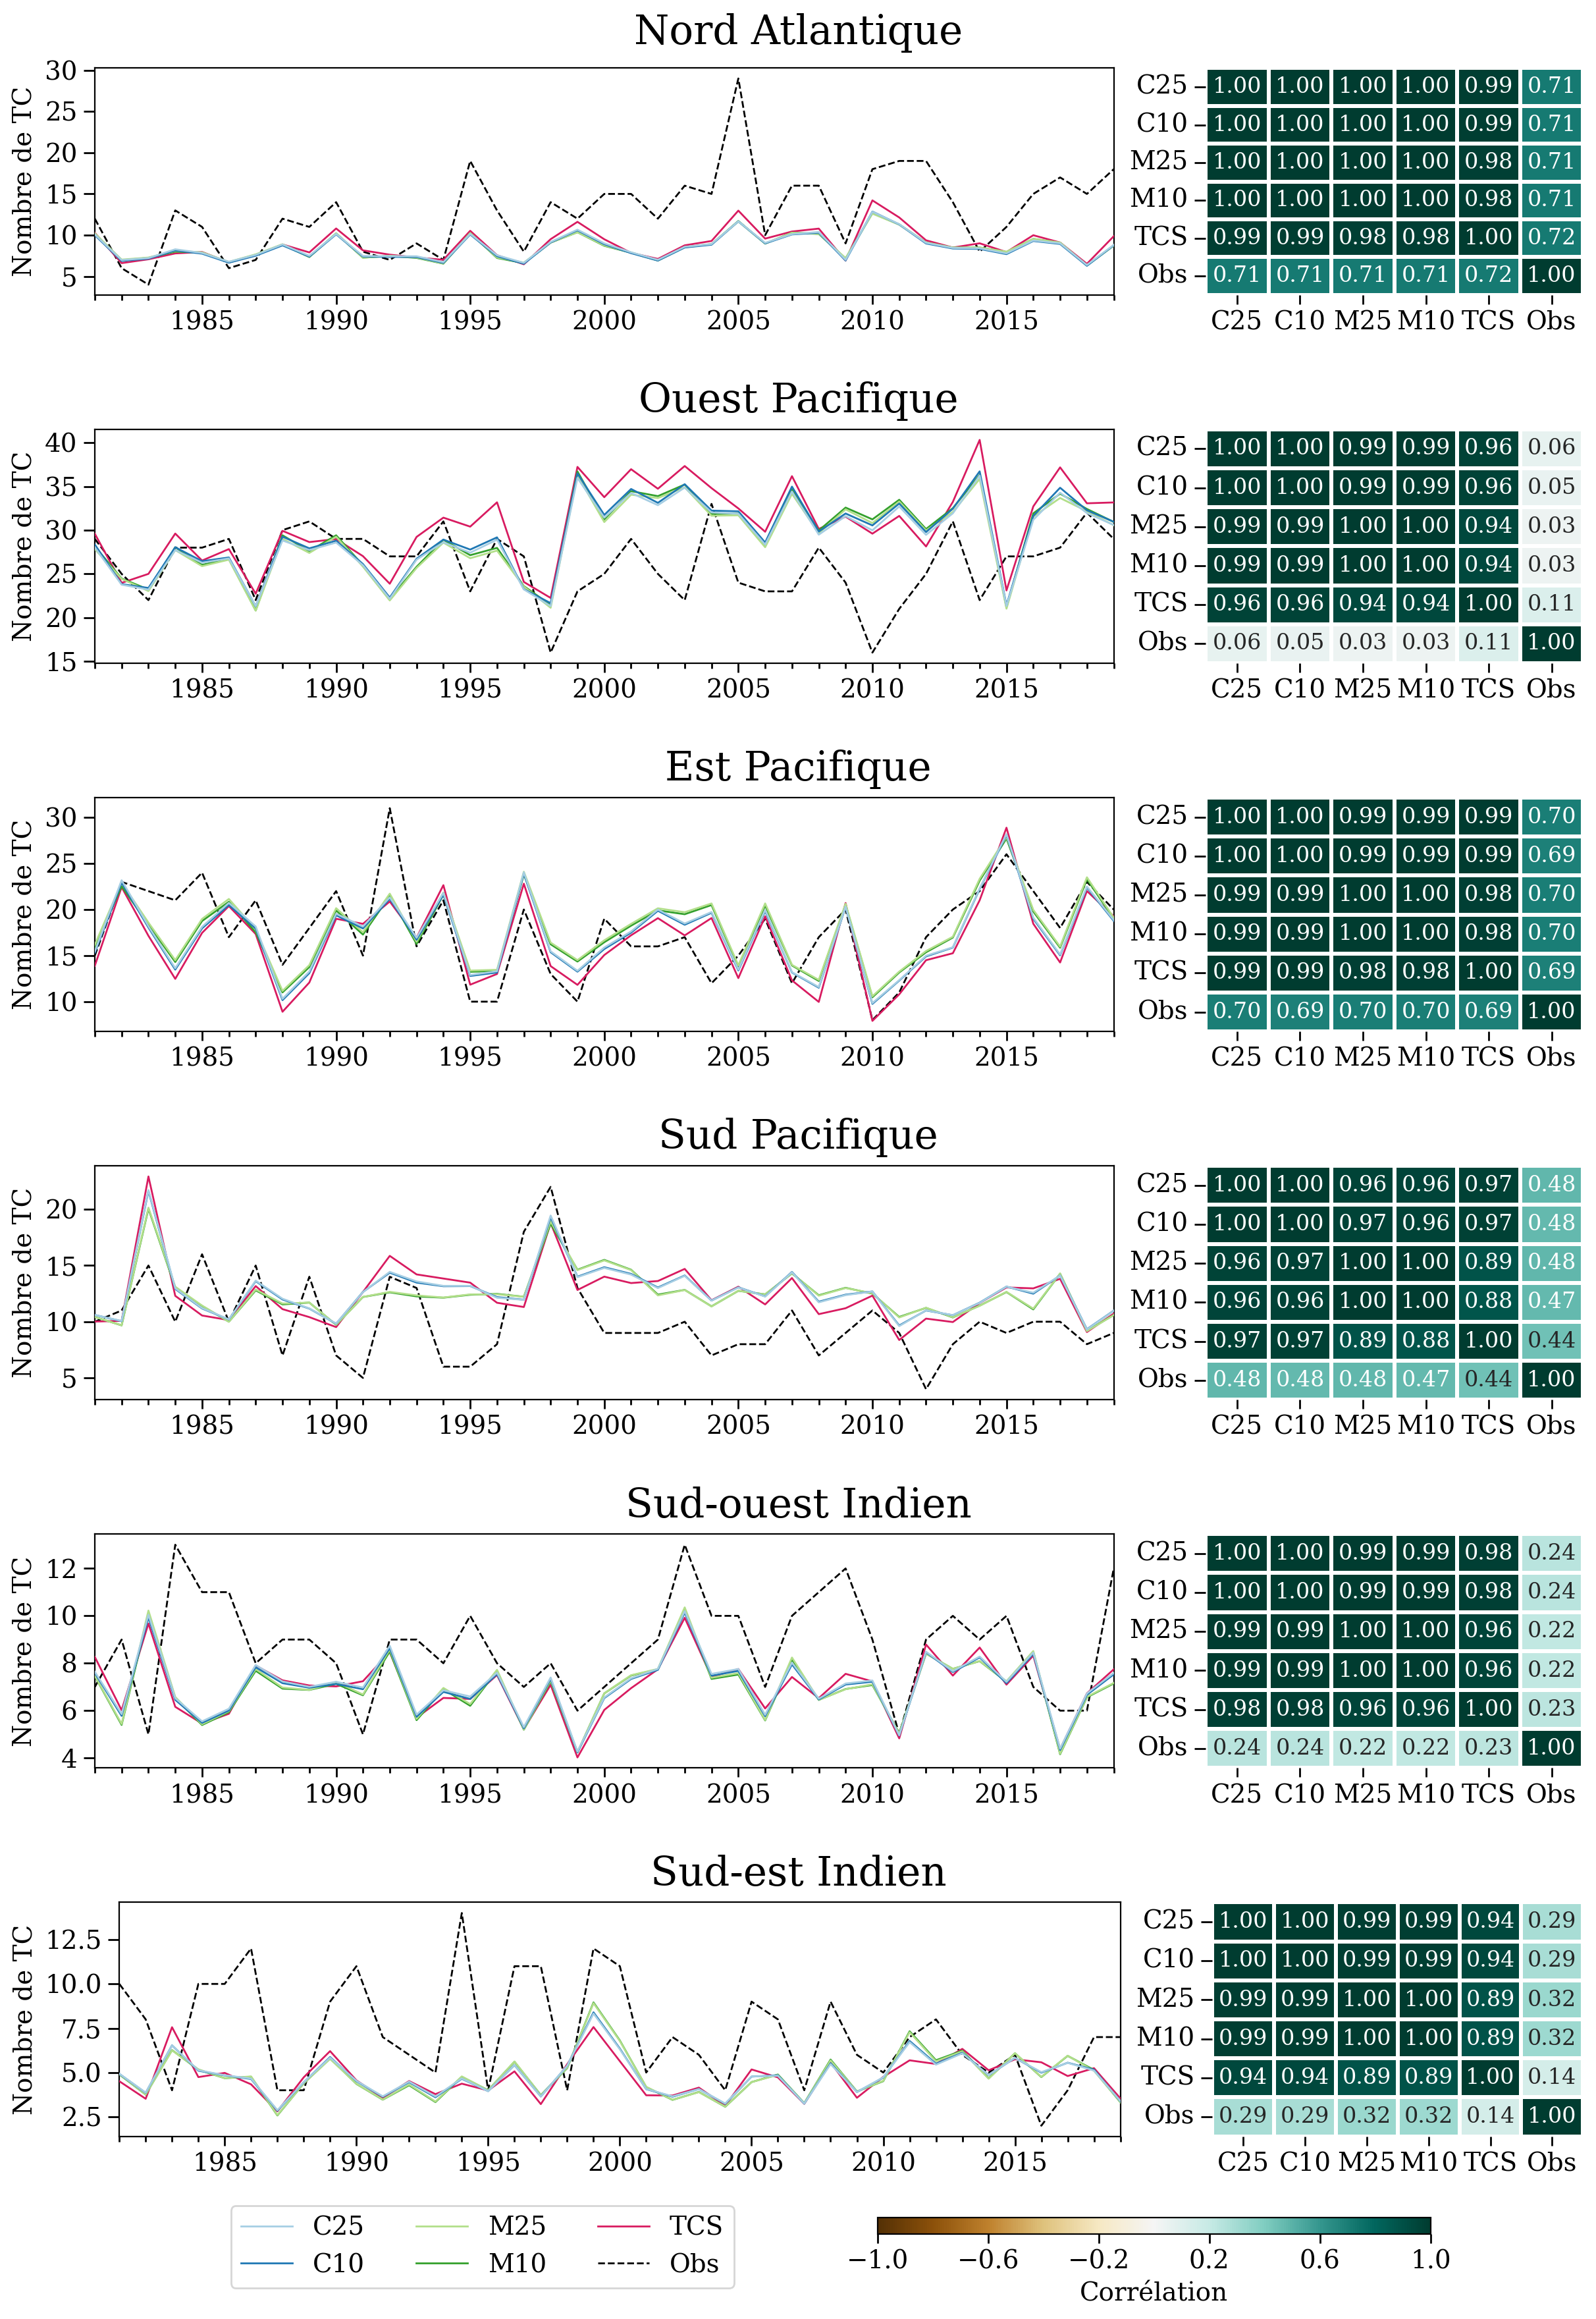
\includegraphics[width=\textwidth]{basin_variability_C25_C10_M25_M10_TCS_obs.png}
    \caption{Variabilité interannuelle du C25, C10, M25, M10, TC et d'IBTrACS, noté \textquote{Obs} pour les six bassins océaniques (lignes), NInd exclu, sur
    les saisons cycloniques de \num{1981} à \num{2019}. Les matrices de corrélation entre indices sont présentées sur la colonne de droite à chaque ligne.}
    \label{fig:variabilite_basin_5_indices}
\end{figure}

Il est immédiatement clair sur la \cref{fig:variabilite_basin_5_indices} que la variaiblité interannuelle inférée par les quatre indices du
\cref{tab:fit_spatial_temporel} est virtuellement inchangée, entre elles, mais aussi par rapport à celle simulée par le TCS. Dans toutes les régions
considérées, les indices climatologiques, C25 et C10 sont légèrement plus proches du TCS que ne le sont les indices mensuels, comme en attestent les matrices de
corrélation (5\ieme~colonne, ou ligne, au choix). Dans les bassins de l'hémisphère nord, la différence est marginale, située entre \num{1e-2} et \num{2e-2}.
L'écart se creuse davantage pour les régions SIndE et SPac, avec un écart de \num{0.05} pour le premier et de \num{0.08} pour le second. C'est en effet pour ce
bassin que la plus grande différence est constatée entre le TCS et un des quatre nouveaux indices, à savoir M10, avec une corrélation de \num{0.88}. La
différence est visible sur les séries temporelles, par exemple entre \num{1991} et \num{1995}, ou encore en \num{2003}. Ces écarts ne peuvent toutefois pas être
qualifiés d'améliorations par rapport aux observations, ni nécessairement de dégradation, tous les indices n'étant que faiblement corrélés à IBTrACS. C'est
également pour le bassin SPac que le plus grand écart est constaté entre les indices climatologiques et mensuels (lignes 3 et 4 contre colonnes 1 et 2, et
réciproquement, de la matrice de corrélation), avec la valeur la plus basse à \num{0.96} pour les paires (M10, C25), (M10, C10) et (M25, C25). Partout ailleurs,
la corrélation est systématiquement de \num{0.99}. Les corrélations entre les paires d'indice de même aggrégation temporelle (climatologique ou mensuelle) mais
de différentes résolutions (c'est à dire M25 avec M10 et C25 avec C10) sont maximales, à \num{1.00} partout. Cela confirme à nouveau que l'impact le plus
notable pour les régression de Poisson se trouve dans l'ajout de variabilité temporelle, comme déjà montré par les
\cref{fig:impact_spatial_temporel,fig:my_fit_meridional}.

Pour ce qui est de la corrélation avec les observations, les nouveaux indices ---~pourtant issus de régression sur ces mêmes données~--- ne se démarquent pas
particulièrement du TCS. Dans le SPac, la corrélation avec IBTrACS est augmentée de \num{0.04} (\num{0.03} pour M10). Dans le SIndE, la corrélation passe de
\num{0.14} à \num{0.29} pour C25 et C10 et à \num{0.32} pour M25 et M10. Une corrélation de \num{0.32} n'est toutefois probablement pas statistiquement
significative. Dans le SPac, la corrélation est augmentée d'environ \num{0.04}, pour C25 et M25, tandis que l'écart avec M10 n'est que de \num{0.03}. Dans le
SIndW, EPac et le NAtl, la corrélation est essentiellement inchangée. Dans le WPac, la corrélation est même dégradée, passant de \num{0.11} pour TCS à un
minimum de \num{0.03} pour M10. Il est cependant certains que des valeurs de corrélation aussi basses ne sont pas significatives. Ce bassin présente la plus
mauvaise corrélation entre les indices et les observations, comme montré précédemment dans le \cref{tab:tcs_cygp_gpi} de la \cref{sec:proprietes_indices}. La
variabilité interannuelle simulée dans ce bassin présente par ailleurs une étonnante rupture de part d'autre de l'année \num{1998} (visible aussi sur la
\cref{fig:tcs_cygp_gpi_variabilite}, et concerne également le GPI). En effet, la fréquence annuelle moyenne des quatre indices C25, C10, M25 et M10 (moyennés
entre eux) avant 1998 est de \num{25.9} TC par an, et monte subitement à \num{32} TC par an post-\num{1998}, soit un écart de \num{6.1} TC par an de part et
d'autre de la rupture, sans présenter de tendances sur ces deux périodes par ailleurs. Après analyse plus approfondie, il est établit que cette rupture est le
résultat d'une inhomogénéité temporelle de l'humidité relative issue de la réanalyse ERA5 sur cette région, sans toutefois en connaître la cause exacte. C'est
notamment pour cela que le CYGP ne subit pas de modification nette de la fréquence annuelle moyenne sur la \cref{fig:tcs_cygp_gpi_variabilite}, ce dernier
n'étant pas fonction de cette quantité. Qu'elle qu'en soit l'origine, ce défaut d'ERA5 constitue une limitation importante de la réanalyse pour tous les indices
de cyclogénèses basés sur l'humidité relative dans la région du Pacifique ouest.

\subsubsection{Apport de l'utilisation de coefficients \textquote{maison}}\label{sec:diagnostique_rang}

Comme vu précédemment, l'indice C25 est le plus proche du TCS du point de vue méthodologique, car construit sur les moyennes climatologiques des observations et
des champs de grande échelle, tous deux interpolés sur une grille de \ang{2.5} de reésolution. Néanmoins, ses coefficients $b$ sensiblement différents du TCS.
C'est notamment le cas du $b_{V_{\mathrm{shear}}}$ et du $b_T$, ainsi que de l'ordonnée à l'origine $b_0$. Étant établi que C25 n'améliore (ni ne modifie
significativement) la variabilité interannuelle (voir \cref{fig:variabilite_basin_5_indices}), et qu'il ne modifie pas non plus la distribution méridionale
moyenne, en particulier dans la région équatoriale (voir \cref{fig:my_fit_meridional}), on peut alors se demander si ces coefficients sont porteurs de
plus-value quelconque par rapport au TCS. Pour le déterminer, on cherche à mesurer dans quelle proportion les indices sont activés aux points de grille et
échéances correspondants à des cyclogénèses observées.

Pour cela, on introduit un nouveau diagnostique indiquant la moyenne et médiane de la distribution des rangs de la valeur prise par un indice, au point de
grille et à la date d'une cyclogénèse observée, relativement aux valeurs prises par cet indice au même point et même mois pour les autres années.
Spécifiquement, pour chaque évènement de cyclogénèse dans notre jeu de données IBTrACS, caractérisé par un point de grille, un mois et une année, nous extrayons
la série temporelle de l'indice en ce point de grille, composée des valeurs au même mois de toutes les années ($n = \num{40}$). Les valeurs composant la série
sont ensuite ordonnées de la plus grande à la plus petite, de façon à connaître le rang de la valeur correspondant à la date de l'évènement observé. Enfin, le
rang est rapporté en un pourcentage, où chacun des rangs parmi les \num{40} vaut \prct{2.5}, constituant donc la distribution des pourcentiles pour toutes les
cyclogénèses observées. La \cref{fig:percentile_genesis_all} présente ces distributions calculées à partir des \num{2789} évènements de
cyclogénèses\footnote{Le/la lecteur·trice aura peut-être remarqué que \num{2789} cyclogénèses sur \num{40} années fait une moyenne bien différente de celle de
\num{84.7} TC par an évoquée à plusieurs reprises dans ce chapitre. La raison à cela provient du fait que certaines observations sont perdues en raison du
masque terre-mer assez conservatif utilisé, puisque l'indice n'est pas défini en ces points.} issues d'IBTrACS entre \num{1980} et \num{2019}, toutes
régions confondues.

\begin{figure}[tp]
    \centering
    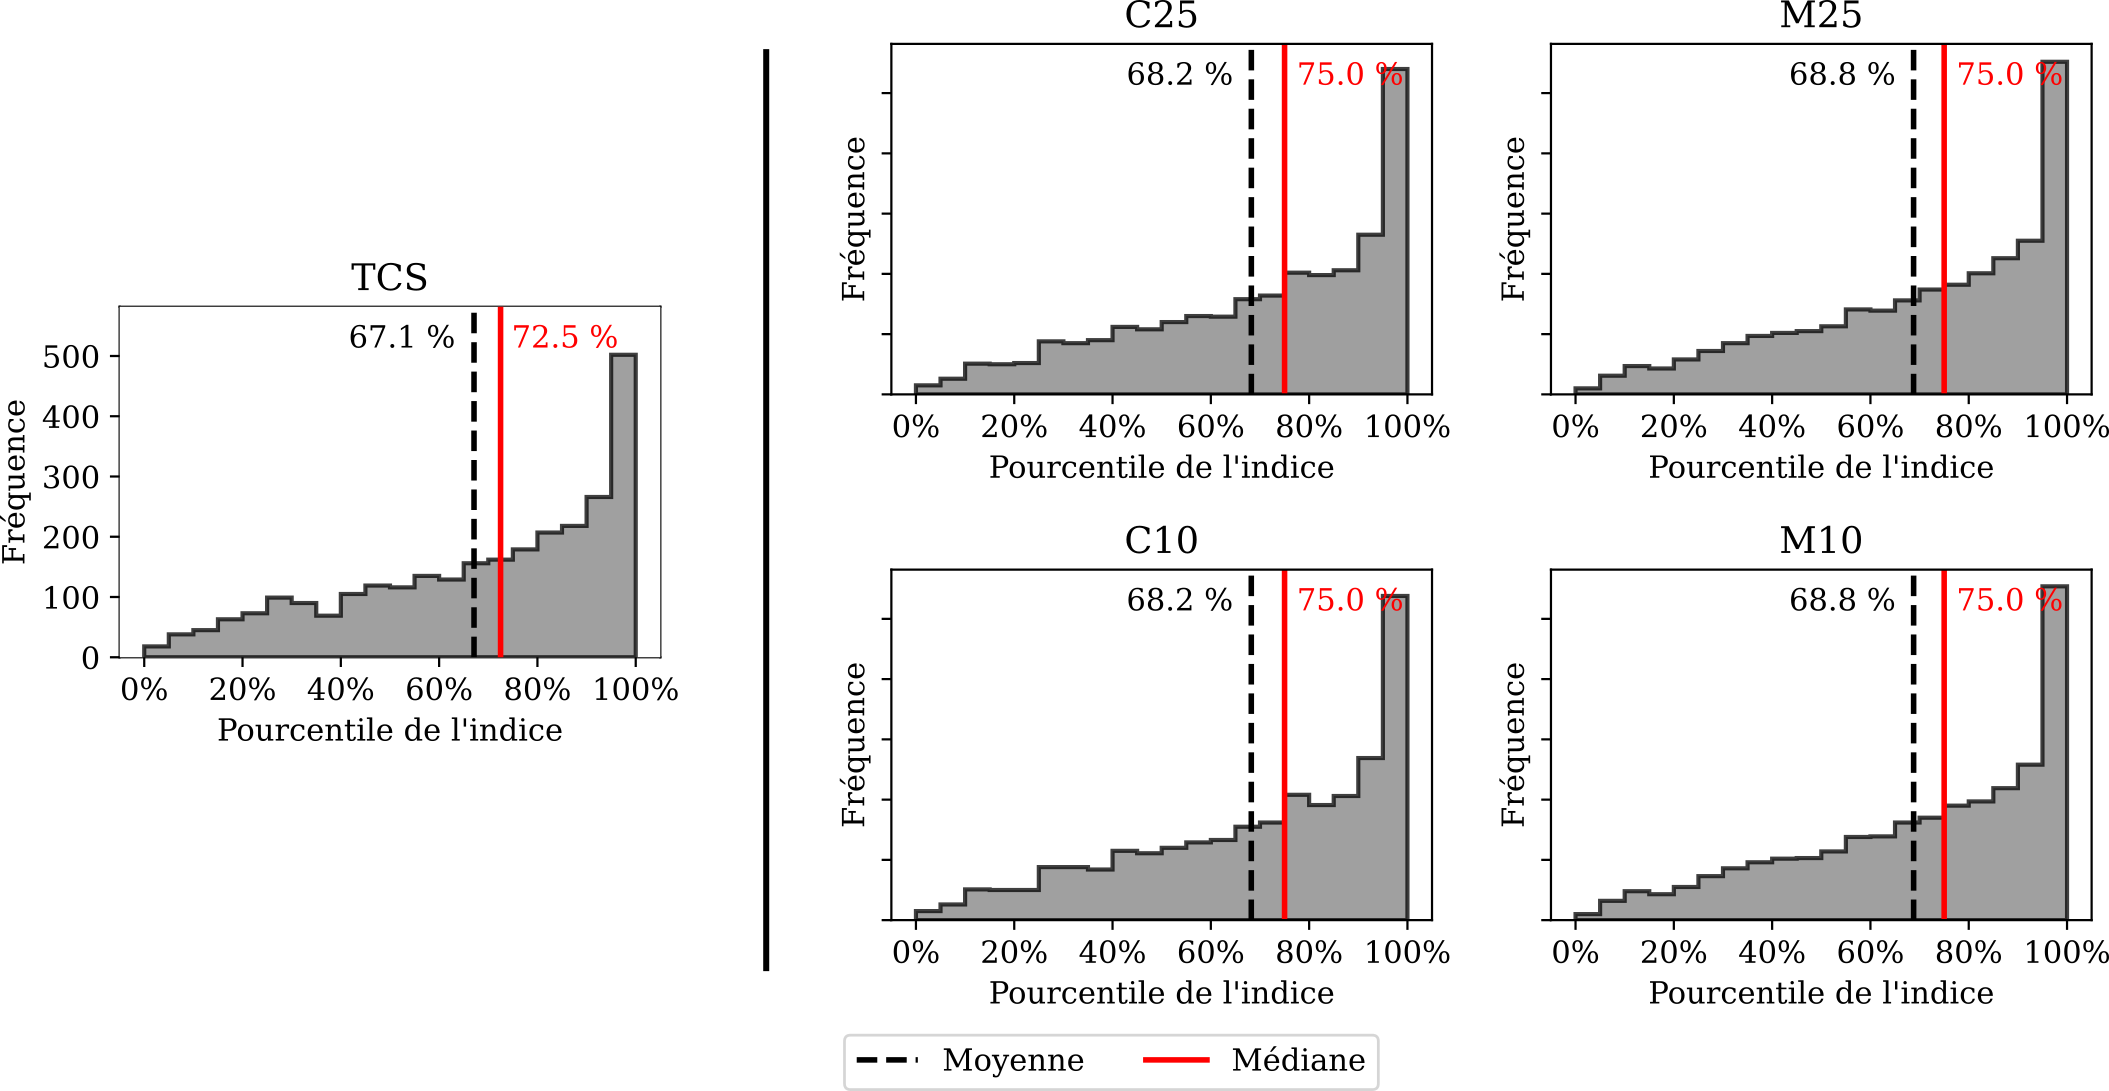
\includegraphics[width=\textwidth]{percentile_genesis_all_5_2.png}
    \caption{Distribution des rangs par rapport aux autres années pour les indices pris aux points de grille et aux dates de cyclogénèses observées. L'encadré à
    gauche de la séparation verticale présente la distribution associée au TCS évaluée sur les cyclogénèses IBTrACS, avec une largeur de \prct{5}. Les quatre
    encadrés à droite de la séparation présentent les distributions pour C25, C10 (1\iere~colonne) et M25 et M10 (2\ieme~colonne).}
    \label{fig:percentile_genesis_all}
\end{figure}

Toutes les distributions présentées sur la \cref{fig:percentile_genesis_all} partagent la même allure, avec une augmentation plus ou moins régulière du nombre
de cas avec des rangs élevés, puis une rupture pour la tranche 95~--~\prct{100}, tranche regroupant le plus grand nombre de cas pour tous les indices. Cette
allure indique que tous les indices présentent une activité supérieure à leur état moyen lorsqu'un évènement a lieu. Un indice ne présentant aucune corrélation
avec l'activité observée à l'échelle du point de grille présenterait au contraire une distribution uniforme. Le TCS, sur la partie gauche de la
\cref{fig:percentile_genesis_all} présente une moyenne et une médiane de \prct{67.1} et \prct{72.5}, respectivement. Un pourcentile de \prct{72.5} correspond à
un rang de \num{11} sur \num{40}. Il y a donc autant de cyclogénèses pour lesquelles le TCS se classe au delà de la \num{11}\ieme~place que de cas où elle se
place avant. Les quatre indices construits dans cette section présentent une médiane à \prct{75}. Cette augmentation de \num{2.5} points de pourcentages est
équivalente à un rang amélioré d'une place, puisque \prct{75} correspond au rang \num{10} sur \num{40}. Notons que les deux indices climatologiques, C25 et C10
partagent la valeur moyenne de \prct{68.2}, tandis que les deux indices mensuels M25 et M10 partagent la valeur de \prct{68.8}. Ainsi, l'apport de variabilité
temporelle dans la régression améliore marginalement la capacité de l'indice à réagir à un évènement de cyclogénèse par rapport aux indices climatologiques.
Cependant, la valeur moyenne comme la médiane de C25 sont supérieures à celles du TCS.

Le \cref{tab:percentiles_indices_all} présente la moyenne et la médiane des quatre indices ainsi que du TCS pour les six régions bassins océaniques. Dans le
NAtl, C25, C10 et M25 partagent les mêmes paramètres de la distribution, avec une moyenne à \prct{64.1}, tandis que M10 atteint une moyenne de \prct{64.4}. Ces
valeurs sont toutes supérieures à la moyenne du TCS, valent \prct{63.2}. La médiane pour les cinq indices est de \prct{70}, inchangée. Dans le WPac, on note une
première amélioration de \prct{68} à \prct{68.1} entre C25 et C10 pour la moyenne, puis \prct{68.8} pour M25 et M10. Là encore, ces valeurs sont supérieures au
TCS. La médiane est également augmentée de \num{2.5} points de pourcentages pour les quatre indices par rapport au TCS. Le bassin EPac constitue un cas un peu
plus particulier, puisqu'il est le seul bassin pour lequel le rang médian perd une place entre les indices mensuels et climatologiques, en dépit d'une hausse
(marginale) de la valeur moyenne. Le bassin SPac atteint un rang médian de \prct{82.5} pour les indices mensuels et de \prct{80} pour les indices
climatologiques, soit respectivement la \num{7}\ieme~et \num{8}\ieme~place. Enfin, pour SIndW et SIndE, les quatre indices présentent tous une médiane \num{2.5}
plus élevée que le TCS, soit un rang amélioré d'une place. Là encore le rang moyen tend à augmenter pour les indices mensuels.

\begin{table}[tb]
    \centering
    \caption{Valeurs moyennes (médianes), exprimées en pourcentage, de la distribution des pourcentiles du rang de l'indice pour les cyclogénèses observées, et
    pour chaque bassin océanique.}
    \begin{tabular}{lrrrrrr}
        \toprule\toprule
        Indice & \multicolumn{6}{c}{Région}\\
        \midrule
               & NAtl & WPac & EPac & SPac & SIndW & SIndE \\
        \midrule 
        C25 & \num{64.1} (\num{70}) & \num{68} (\num{75}) & \num{66.1} (\num{72.5}) & \num{74.7} (\num{80}) & \num{71.8} (\num{77.5}) & \num{67.9} (\num{72.5}) \\
        C10 & \num{64.1} (\num{70}) & \num{68.1} (\num{75}) & \num{66.1} (\num{72.5}) & \num{74.6} (\num{80}) & \num{71.8} (\num{77.5}) & \num{67.9} (\num{72.5}) \\
        M25 & \num{64.1} (\num{70}) & \num{68.8} (\num{75}) & \num{66.4} (\num{70}) & \num{75.3} (\num{82.5}) & \num{72.3} (\num{77.5}) & \num{68.5} (\num{72.5}) \\
        M10 & \num{64.4} (\num{70}) & \num{68.8} (\num{75})& \num{66.4} (\num{70}) & \num{75.4} (\num{82.5}) & \num{72.3} (\num{77.5}) & \num{68.8} (\num{72.5}) \\
        \midrule
        TCS & \num{63.2} (\num{70}) & \num{66.6} (\num{72.5}) & \num{65.5} (\num{70}) & \num{74.2} (\num{80}) & \num{69.9} (\num{75}) & \num{66.5} (\num{70}) \\
        \bottomrule
    \end{tabular}
    \label{tab:percentiles_indices_all}
\end{table}

Pour résumer, tous les indices présentent un rang médian au moins égal à ceux du TCS, tandis que le rang moyen est toujours supérieur. Les indices construits
sur les champs mensuels, M25 et M10 présentent systématiquement un rang moyen amélioré par rapport aux indices C25 et C10, à l'exception de M25 dans le NAtl qui
demeure inchangé. Le rang médian est lui souvent inchangé pour les indices mensuels, à l'exception du bassin SPac où M25 et M10 prennent tous deux une place,
tandis qu'ils en perdent une dans le bassin EPac.

\subsection{Conclusion}

Dans cette section, quatre indices de cyclogénèses ont été construits en reproduisant la méthodologie de \textcite{tippett_poisson_2011}, à savoir la régression
de Poisson (voir \cref{sec:apport_res_methodes}), en utilisant les mêmes prédicteurs de grande échelle que sont la vorticité absolue bornée, le cisaillement
vertical du vent, l'humidité relative et la SST relative. Ces indices sont construits entre d'une part la réanalyse atmosphérique ERA5, et de l'autre la base de
données observationelle IBTrACS. Outre la période temporelle utilisée ici, différente de celle utilisée pour déterminer les coefficients $b$ du TCS, les indices
nouvellement définis se distinguent par la résolution spatiale des champs (de grande échelle, comme de l'activité cyclonique observée), ainsi que par la
résolution temporelle. En effet, deux des indices sont construits sur les moyennes climatologiques des champs atmosphériques et des observations IBTrACS (C25 et
C10), tandis que les deux autres sont construits directement à partir des moyennes mensuelles (M25 et M10), ce qui revient à apporter de la variabilité
temporelle à plus haute fréquence dans la régression statistique. De la même façon, deux indices sont construits sur des champs à la résolution grossière de
\ang{2.5} (C25 et M25), tandis que les deux autres sont établis à \ang{1} de résolution horizontale (C10 et M10). En pratique, les quatre indices se
distinguent, entre eux mais aussi du TCS, par les coefficients $b$ qui les caractérisent, puisque tous sont évalués et comparés sur les champs mensuels ERA5 à
\ang{1} de résolution, indépendamment de la manière dont la régression a été menée.

Comme attendu, les coefficients de C25 sont les plus proches de TCS, avec notablement une sensibilité diminuée à la SST relative, et au contraire une
sensibilité accrue au cisaillement vertical. S'il est possible qu'une partie de ces différences provienne de l'utilisation d'un jeu de données d'origine
différente, il semblerait que la période temporelle utilisée joue un rôle important, puisque ces deux coefficients s'éloignent du TCS au fur et à mesure que la
période temporelle est lointaine de celle utilisée par \textcite{tippett_poisson_2011} (\num{1961}~--~\num{2000}). Si cette tendance venait à être confirmée, le
décalage si rapide dans le temps des coefficients de l'indice questionnerait sérieusement le bienfondé de l'application des indices de cyclogénèses pour l'étude
du climat futur. L'apport de la résolution spatiale accrue, comme celui de l'ajout de variabilité temporelle dans la régression se traduisent tous deux par une
diminution de l'activité à proximité immédiate de l'équateur, au profit des régions de basses latitudes immédiatement attenantes. L'effet de la variabilité
temporelle est dominant, les deux étant séparés d'un ordre de grandeur (voir \cref{sec:repartition_geographique}, \cref{fig:impact_spatial_temporel}). De plus,
l'utilisation de données mensuelles dans la régression produit un coefficient associé à la vorticité absolue bornée augmenté de plus de \prct{30}. Il apparaît
que cet ordre de grandeur de $b_\eta$, à environ \num{1.39} contre \num{1.03} pour le TCS, permette la correction quasi complète du biais équatorial dont le TCS
souffre sinon (voir \cref{fig:my_fit_meridional}).

Si les coefficients $b$ des indices définis par régression de Poisson ne sont que modérément robustes ---~selon la variable considérée~--- la variabilité
interannuelle inférée par ces mêmes indices l'est quant à elle très fortement. En effet, ni la résolution horizontale accrue, ni l'introduction de variabilité
temporelle à plus haute fréquence dans la régression, et donc les variations de coefficients qui en résultent, ne changent de manière significative la
variabilité interannuelle. Cela suggère par conséquent que le choix des prédicteurs est le facteur principal influençant la variabilité interannuelle, bien plus
que les coefficients de pondération qui leur sont associés. Par ailleurs, cette analyse a mis en évidence un problème d'homogénéité temporelle dans le champ
d'humidité relative de la réanalyse ERA5 dans la région du Pacifique ouest, résultant en une modification brutale de la fréquence moyenne annuelle de part et
d'autre de l'année \num{1998}. Ce problème compromet considérablement l'utilisation d'indices définis en fonction de l'humidité relative pour l'étude de
l'activité cyclonique dans cette région avec ERA5. Ce problème est également visible dans l'analyse qui est faite dans la \cref{sec:proprietes_indices},
notamment pour le GPI, et n'est donc pas limité au TCS et à ses variantes.

En dépit de l'effet particulièrement marginal de la résolution spatiale et temporelle sur la variabilité interannuelle, il est montré dans la
\cref{sec:diagnostique_rang} que l'estimation de nouveaux coefficients $b$, supposément mieux adaptés au jeu de donnée cible, apporte tout de même une
plus-value. Le nouveau diagnostique qui y est introduit, consistant en la mesure des paramètres de la distribution des rangs des valeurs prises par l'indice aux
points de grille et aux dates des cyclogénèses observées, montre en effet une réactivité systématiquement accrue pour les indices construits sur nos jeux de
données, par rapport aux coefficients du TCS. Dans le contexte précis de l'étude réalisée ici, le gain est cependant marginal, et il n'est en outre pas certain
que cette légère amélioration de la cohérence entre l'indice et les observations justifie à elle seule la quantité de travail requise à l'estimation de nouveaux
coefficients.

\section{Indice de cyclogénèse régional}\label{sec:indice_regional}

Après avoir défini de nouveaux indices construits à partir de champs à différentes résolutions spatiales et temporelles dans la
\cref{sec:apport_res_temporel_spatial}, on s'intéresse dans cette question à la construction d'indices de cyclogénèses régionaux. Comme précédemment, les
indices régionaux sont construits par régression de Poisson, dont le fonctionnement est détaillé dans la \cref{sec:apport_res_methodes}. Toutefois, au lieu de
déterminer une relation entre l'environnement de grande échelle et l'activité cyclonique observée à l'échelle globale, la régression est appliquée à l'échelle
du bassin cyclonique. Les coefficients $b$ de la régression se s'interprétant comme des sensibilités, on s'intéresse notamment à l'information apportée par les
différentes valeurs prises par chacun des coefficients dans chacune des régions géographiques.

\subsection{Méthodes}

Pour cet exercice, les bassins océaniques usuels sont utilisés, c'est à dire ceux présentés sur la \cref{fig:impact_spatial_temporel}. Les premières
observations des systèmes issus d'IBTrACS, version 4, sont assimilés aux cyclogénèses (vecteur $Y$ de la relation \ref{eq:poisson_reg}), dès lors que ces
systèmes atteignent à un moment de leur cycle de vie le stade de tempête tropicale ou subtropicale. Comme précédemment, on se limite pour la régression aux
données entre \num{1980} et \num{2019}. Les indices régionaux sont construits selon la même méthodologie que pour l'indice M10 décrit dans la
\cref{sec:apport_res_methodes}, c'est à dire sur les champs de grande échelle ERA5 mensuels à \ang{1} de résolution. En effet, comme vu précédemment,
l'introduction de variabilité à plus haute fréquence dans la régression peut apporter de l'information qui serait sinon manquée avec des moyennes
climatologiques. Par ailleurs, bien que les indices basés sur des champs mensuels n'impactent pas la variabilité interannuelle simulée, il semble déraisonnable
d'espérer pouvoir l'améliorer sans introduire de variabilité temporelle dans la régression. Quant à la résolution, nous utilisons les champs à \ang{1} de
résolution, malgré l'impact marginal du passage depuis \ang{2.5}, car le masque terre-mer à \ang{2.5} risquerait de réduire trop fortement le nombre de points
de grille utiles pour des régression réalisées à cette échelle. Les mêmes prédicteurs que pour le TCS sont utilisés, et décrits dans la
\cref{sec:apport_res_methodes}, de façon à voir la sensibilité de l'activité cyclonique de chaque bassin à ces derniers.

Une fois les coefficients déterminés, les relations établies pour chaque bassin sont appliquées aux champs mensuels ERA5 à \ang{1}. La calibration des indices
régionaux est faite de façon à ce que l'intégrale de chaque indice régional soit égal à l'intégrale de l'indice M10 sur ce bassin (ce dernier étant calibré sur
IBTrACS à l'échelle globale).


\subsection{Coefficients régionaux}\label{sec:lm10_coefficients}

Le \cref{tab:coefs_fit_bassin} présente les coefficients $b$ pour les six régression régionales. Comme pour la \cref{sec:apport_res_temporel_spatial},
l'interprétation de l'ordonnée à l'origine $b_0$ est mise de côté. Au delà de ce coefficient, les régressions à l'échelle du bassin mettent en évidence des
sensibilités aux variables de grande échelle très différentes selon les bassin, variant du simple au double pour certaines variables, et de manière plus modeste
pour d'autres.

\begin{table}[htpb]
    \centering
    \caption{Estimation des coefficients $b$ et de leur erreur standard pour chaque régression faite à l'échelle du bassin océanique. Les deux dernières lignes
    présentent les coefficients pour l'indice M10 de la \cref{sec:apport_res_temporel_spatial} et du TCS. La colonne Fréquence indique le nombre annuel moyen de
    TC pour les indices régionaux, calibrés pour simuler la même fréquence que l'indice M10 dans chacun des bassins.}
    \label{tab:coefs_fit_bassin}

    \resizebox{\textwidth}{!}{
    \begin{tabular}{lrrrrrr}
       \toprule\toprule 
       \multicolumn{1}{c}{Bassin} & \multicolumn{5}{c}{Coefficients} & \multicolumn{1}{c}{Fréquence}\\
       \midrule
               & $b_0$ & $b_{\eta}$ & $b_{V_{\mathrm{shear}}}$ & $b_H$ & $b_T$ &  \\
       \midrule
       NAtl    & \mypm{-17.3713}{0.735} & \mypm{2.1677}{0.163} & \mypm{-0.0594}{0.010} & \mypm{0.0651}{0.004}  & \mypm{0.3313}{0.022} & $\num{8.6}$  \\
       WPac    & \mypm{-14.2693}{0.303} & \mypm{0.9547}{0.045} & \mypm{-0.0715}{0.008} & \mypm{0.0760}{0.003}  & \mypm{0.4860}{0.041} & $\num{29.2}$ \\ 
       EPac    & \mypm{-16.2217}{0.409} & \mypm{1.5829}{0.076} & \mypm{-0.0805}{0.009} & \mypm{0.0748}{0.004}  & \mypm{0.6970}{0.042} & $\num{17.7}$  \\
       SPac    & \mypm{-15.6428}{0.555} & \mypm{1.5562}{0.115} & \mypm{-0.1282}{0.016} & \mypm{0.0666}{0.006}  & \mypm{0.5208}{0.055} & $\num{12.5}$   \\
       SIndW   & \mypm{-16.7210}{0.578} & \mypm{1.8837}{0.130} & \mypm{-0.0590}{0.014} & \mypm{0.0686}{0.005}  & \mypm{0.5779}{0.102} & $\num{7}$   \\
       SIndE   & \mypm{-15.0059}{0.643} & \mypm{1.5269}{0.155} & \mypm{-0.0706}{0.014} & \mypm{0.0640}{0.005}  & \mypm{0.4298}{0.052} & $\num{4.8}$   \\
       \midrule
       %\multicolumn{1}{c}{Indices} & \multicolumn{5}{c}{Coefficients} & \multicolumn{3}{c}{Détails}\\
       \multicolumn{7}{c}{Indices de Référence}\\
       \midrule
       M10  & \mypm{-15.0496}{0.162} & \mypm{1.3968}{0.032} & \mypm{-0.0960}{0.004} & \mypm{0.0718}{0.002}  & \mypm{0.4142}{0.015} & $\num{84.7}$ \\
       TCS  & $\num{-5.8}$     & $\num{1.03}$   & $\num{-0.15}$   & $\num{0.05}$    & $\num{0.56}$   & $\num{84.7}$  \\
       \bottomrule
    \end{tabular}
    }
\end{table}

L'humidité relative à \hPa{600} fait partie des variables pour lesquelles la sensibilité de la fréquence attendue de cyclogénèses est relativement stable pour les
différents bassins. Les valeurs de $b_H$ varient entre \num{0.064} pour le SIndE et \num{0.076} pour le WPac. Toutefois, la valeur du coefficient dans le WPac
peut être influencée par la rupture temporelle dans le champ d'humidité relative mise en évidence précédemment. La deuxième valeur la plus grande est atteinte
pour le EPac avec \num{0.0748}. Cette plage de valeur correspond donc à une sensibilité de l'ordre de \prct{6.4} à \prct{7.5} pour un changement unitaire de
l'humidité relative. Les valeurs $b_H$ sont inférieures à celle de M10 pour quatre des 6 régions géographiques, avec seul le pacifique nord (ouest comme est)
situé au dessus. Le $b_H$ moyen sur les six régions est d'environ \num{0.0692}, soit également inférieur à M10. Dans ce dernier, il est possible que le bassin
NInd contribue à augmenter le $b_H$ global, ce bassin n'étant pas intégré aux régression locales pour cause de données observationelles manquantes. L'erreur
standard relative de $b_H$ pour les régression régionales se situe entre \prct{4} et \prct{9} de la moyenne estimée.

Les coefficients associés au cisaillement vertical, $b_{V_{\mathrm{shear}}}$ présentent également une faible dispersion, à l'exception du SPac. Dans tous les
autres bassins, ce coefficient se situe entre \num{-0.059} (SIndW) et \num{-0.0805} (EPac). Dans le SPac, ce coefficient atteint \num{-0.1282}. La différence
avec les cinq autres bassins est donc importante. La valeur moyenne de $b_{V_{\mathrm{shear}}}$ vaut environ \num{-0.068}, soit un peu plus de la moitié du
coefficient du SPac. L'erreur standard relative est maximale pour le SIndW, à près de \prct{24}, suivi du bassin SIndE à environ \prct{20}. En comparaison,
l'erreur standard relative pour le bassin SPac n'est que de \prct{12}. Ici encore, la moyenne des $b_{V_{\mathrm{shear}}}$, incluant le SPac
(\sim~\num{-0.0782}) est éloignée de la valeur de l'indice M10. Tous les bassins, à l'exception du SPac, indiquent en effet une sensibilité diminuée au
cisaillement vertical par rapport au $b_{V_{\mathrm{shear}}}$ global de M10. L'absence du bassin NInd dans les régression locales peuvent aussi expliquer au
moins en partie cette différence, le cisaillement étant un facteur très déterminant dans cette région \parencite{gray_global_1968}.

La sensibilité à la SST relative présente quant à elle une plus grande variabilité spatiale. La plus grande sensibilité à la SST relative est notée pour le
bassin EPac, avec \num{0.697}, avec une erreur standard relative de \prct{6}. La SST dans ce bassin est particulièrement impactée par les épisodes El Niño et El
Niña, puisque c'est dans ce bassin que l'anomalie de température de surface de l'océan y est diagnostiquée. Entre ERA5 et IBTrACS, nous notons une corrélation
entre l'activité observée et l'indice ONI ---~diagnostique opérationnel du mode de variabilité El Niño/Niña, défini comme l'anomalie de température sur trois
mois glissants entre \ang{170}W et \ang{120}W en longitude et \ang{5}S et \ang{5}N en latitude~--- à l'échelle du bassin EPac de \num{0.54}. Le lien entre ce
mode de variabilité et l'activité cyclonique est également documenté dans la littérature \parencite{camargo_use_2007,lin_enso_2020}. Une forte
sensibilité du modèle de Poisson à la SST relative dans ce bassin était alors attendue. À l'inverse, la sensibilité la plus faible à la SST relative est obtenue
pour le bassin NAtl.

Si le bassin NAtl présente la plus faible sensibilité à la SST relative, et la deuxième plus faible sensibilité au cisaillement vertical, juste derrière le
bassin SIndW, la régression indique cependant une très forte sensibilité à la vorticité absolue bornée $\eta$. En effet, $b_\eta$ pour le NAtl atteint la valeur
record de \num{2.1677}, loin devant tous les autres bassins. Pour une telle valeur, l'approximation $e^{b_\eta} \approx 1 + b_\eta$ n'est absolument pas valide.
Ici, la fréquence attendue est modifiée d'un facteur $e^{b_\eta}$ environ égal à \num{8.7} pour un changement unitaire de la vorticité absolue bornée. La
vorticité apparaît donc dans la régression comme le facteur le plus déterminant pour expliquer la fréquence d'occurrence des TC dans ce bassin. Dans le WPac,
$b_\eta$ est au contraire à sa valeur la plus basse comparée aux autres régions, à \num{0.9547}. Notons que tous les autres bassins présentent un $b_\eta$ sinon
supérieur à la valeur de M10, situé entre \num{1.5} et \num{1.6} pour les bassins EPac, SPac, SIndW et SIndE, d'environ \num{1.88} pour le bassin SPac.

\subsection{Effet sur la répartition spatiale}\label{sec:lm10_effet_spatial}

De manière analogue à la \cref{sec:apport_resultat}, nous évaluons ici l'impact des coefficients $b$ différents sur la répartition spatiale de l'activité pour
chacun des bassins. Par commodité, désignons par le nom de LM10 (comme \textquote{Local}) l'ensemble des indices régionaux, dont l'agrégation forme un indice
pseudo-global. LM10 peut en effet être vu comme une déclinaison régionale de l'indice M10. LM10 est caractérisé par ses coefficients $b$, qui eux-mêmes sont
fonction du bassin géographique. À la différence de M10, LM10 est indéfini en dehors des six bassins listés dans le \cref{tab:coefs_fit_bassin}. La
\cref{fig:diff_LM10_M10} présente la moyenne annuelle, exprimée en TC par \ang{1}$\times$\ang{1} par an, de la quantité $\mathrm{LM10} - \mathrm{M10}$. Puisque
LM10 est calibré pour produire dans chaque bassin la fréquence annuelle moyenne de M10, l'intégrale des cartes de la \cref{fig:diff_LM10_M10} sont égales à
\num{0}.

\begin{figure}[tp]
    \centering
    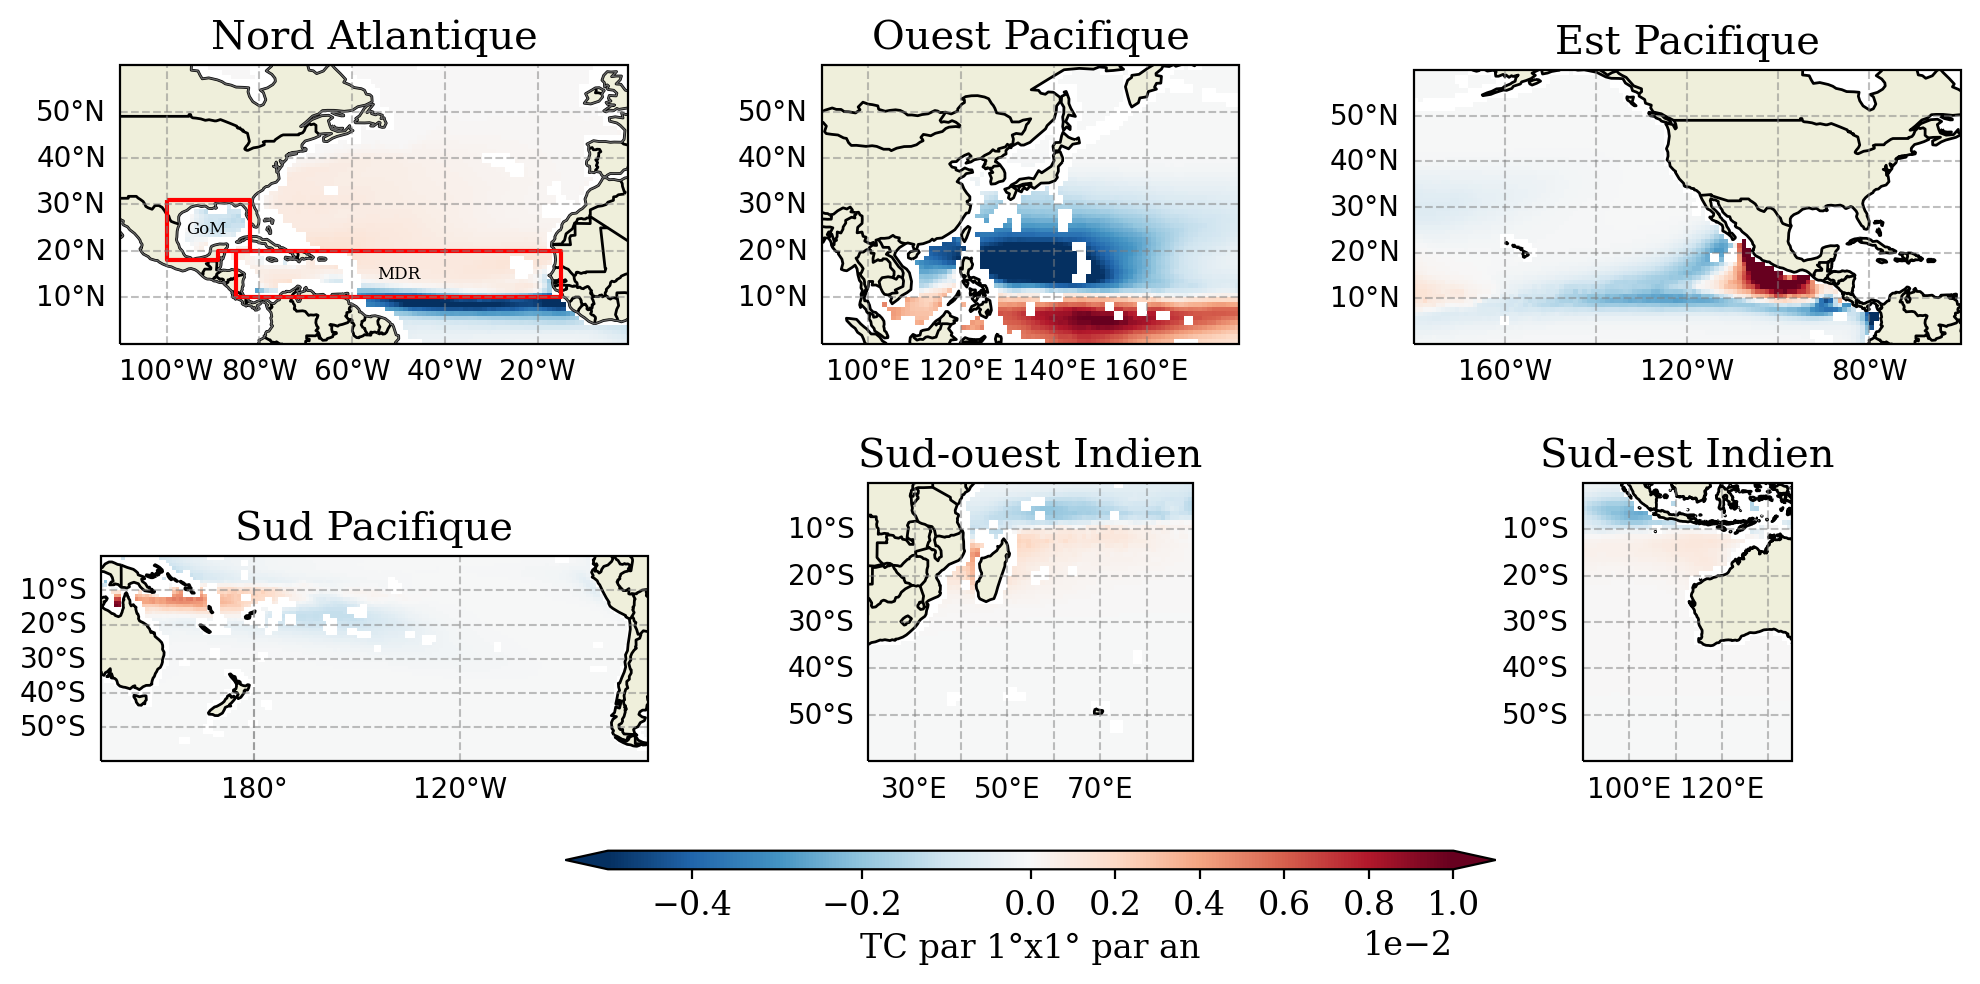
\includegraphics[width=\textwidth]{diff_LM10_M10.png}
    \caption{Carte du déport d'activité pour chaque bassin entre l'indice régional et M10. Un changement positif indique une activité simulée accrue pour l'indice
    régional par rapport à M10. L'intégrale pour chaque bassin est nulle, par construction. Pour le bassin Nord Atlantique, les boîtes rouges indiquent les deux
    sous-régions, que sont le GoM et la MDR, concentrant la majorité des cyclogénèses dans le bassin.}
    \label{fig:diff_LM10_M10}
\end{figure}

Le bassin NAtl est caractérisé par un fort déport de l'activité inférée par M10 à proximité de l'équateur dans tout le reste du bassin, à l'exception du Golf du
Mexique (Encadré en rouge, GoM), qui voit lui aussi une diminution relative dans LM10. Rappelons que la \cref{sec:apport_res_temporel_spatial} a mis en évidence
le rôle du coefficient $b_\eta$ dans le décalage méridional de l'activité inférée. Dans la mesure où LM10 présente un $b_\eta$ encore plus important, il est
permis de penser que c'est cette sensibilité accrue à la vorticité absolue de LM10 qui est à l'origine de la diminution de l'activité sur la bande entre
\ang{5}N et \ang{10}N. Cette baisse se fait notamment au bénéfice de la région de développement principale (MDR), également encadrée en rouge sur la carte du
NAtl de la \cref{fig:diff_LM10_M10}. Dans la MDR, LM10 simule environ \num{3.97} TC par an, contre \num{3.8} TC par an pour M10. Dans le GoM, LM10 simule en
revanche \num{1.07} TC par an contre \num{1.12} TC par an pour M10. À titre de référence, les données de cyclogénèses IBTrACS utilisées ici indiquent \num{5.64}
TC par an dans la MDR et \num{1.87} TC par an dans le GoM. Ainsi, LM10 simule une activité légèrement plus proche d'IBTrACS dans la MDR, mais dégradée par
rapport à M10 dans le GoM. L'origine de la diminution dans le GoM est incertaine, mais au vue des coefficients du \cref{tab:coefs_fit_bassin}, il semble
probable que ce soit principalement le résultat de la baisse de sensibilité à la SST relative, et peut-être aussi dans une moindre mesure à la diminution de la
sensibilité à l'humidité relative (comparativement moindre), dans la mesure où la diminution de la sensibilité au cisaillement vertical ne saurait expliquer une
baisse de l'activité. Notons que la racine carrée de l'erreur quadratique moyenne (\textit{Root Mean Squared Error}, RMSE) entre la moyenne annuelle d'IBTrACS
---~lissée au préalable avec un filtre gaussien à \ang{1} d'écart-type~--- et la moyenne annuelle de l'indice passe de \num{3.3e-3} avec M10 à \num{3.1e-3} avec
LM10, indiquant donc dans une meilleure (marginalement) proximité de LM10 avec IBTrACS.

Dans le WPac, la carte des différences ne présente aucune ambigüité. L'activité dans LM10 est augmentée en dessous de \ang{10}N, et diminuée au delà, en
particulier en Mer de Chine Méridionale et mer des philippines, où la basse est maximale. Le déport vers l'équateur peut s'expliquer au moins en partie par un
$b_\eta$ particulièrement bas, en dessous de \num{1}, plus bas encore que celui du TCS. C'est ce paramètre qui le distingue le plus de M10. Quoiqu'il en soit,
la répartition spatiale de LM10 dans ce bassin est plus proche d'IBTrACS que ne l'est M10. En effet, entre \ang{0} et \ang{10}N, IBTrACS indique \num{9.83} TC
par an, M10 simule \num{6.78} TC par an tandis que LM10 en simule \num{9.61} TC par an. Cela implique également que M10 surestime l'activité entre \ang{10}N et
\ang{60}N, avec \num{22.3} TC par an contre \num{16.3} TC par an pour IBTrACS, alors que LM10 est par conséquent plus proche des observations, avec \num{19.72}
TC par an. La régression sur le bassin WPac permet une meilleure ressemblance avec la répartition spatiale de l'activité observée dans IBTrACS. Le RMSE
est en effet réduit de \num{9.5e-3} avec M10 à \num{7.9e-3} avec LM10. L'amélioration de la cohérence spatiale est plus importante que pour le NAtl.

Dans le bassin EPac, LM10 concentre l'activité le long des côtes du Mexique, avec également une légère augmentation à l'extrémité l'ouest du domaine, de part et
d'autre de \ang{10}N. Comme pour les autres bassins, ce déport favorise la ressemblance avec les observations, avec un RMSE passant de \num{8.3e-3} à \num{7.6e-3} pour
LM10. LM10 y parvient en modifiant principalement la sensibilité à la SST $b_T$ relative (accrue) et à la vorticité $b_\eta$ (également accrue).

Pour les trois bassins de l'hémisphère sud, l'effet de la régression locale sur la répartition spatiale de l'activité est bien moindre que dans les bassins de
l'hémisphère nord. Dans le SIndW, l'activité est déportée autour de Madagascar, et dans le Canal du Mozambique. Le RMSE avec IBTrACS est essentiellement
inchangé, avec un effet de l'ordre de \num{1e-6}. Dans le SIndE, un constat similaire est fait, avec une baisse entre \ang{0} et \ang{10}S puis une légère
augmentation entre \ang{10}S et \ang{20}S. Le RMSE est modifié de \num{1e-4}, du côté d'une dégradation de LM10 par rapport à M10. Dans le SPac, l'activité est
accrue entre \ang{10}S et \ang{20}S, dans la Mer de Corail, jusqu'à \ang{180}. Comme pour le SIndE, l'erreur quadratique moyenne est accrue avec LM10, passant
de \num{3.3e-3} à \num{4e-3}. Notons enfin que la dissymétrie dans l'impact sur la répartition géographique de LM10 par rapport à M10, avec des changements plus
importants dans l'hémisphère nord que dans l'hémisphère sud, est cohérente avec les \cref{fig:tcs_cygp_gpi_zonal,fig:my_fit_meridional}, des sections
précédentes montrant toutes deux une distribution méridionale de l'activité moyenne plus éloignée des observations dans l'hémisphère nord que dans l'hémisphère
sud.

\subsubsection{Variabilité interannuelle}\label{sec:lm10_corr}

Il a été montré dans la \cref{sec:apport_res_temporel_spatial} que les coefficients $b$ de l'indice n'influent que très peu la variabilité interannuelle inférée
par l'indice. Il n'est par conséquent pas attendu que LM10 se démarque de M10 ou encore du TCS pour ce qui est de la corrélation entre la variabilité
interannuelle et les observations. La \cref{fig:corr_lm10_m10_ibt} présente les matrices de corrélation de la variabilité interannuelle entre LM10, M10, TCS et
IBTrACS entre les saisons 1981 et 2019, calculés selon la méthodologie de la \cref{sec:variabilite_5_indices}. Les séries temporelles sont omises car
indiscernables de celles présentées sur la \cref{fig:variabilite_basin_5_indices}.

\begin{figure}[htb]
    \centering
    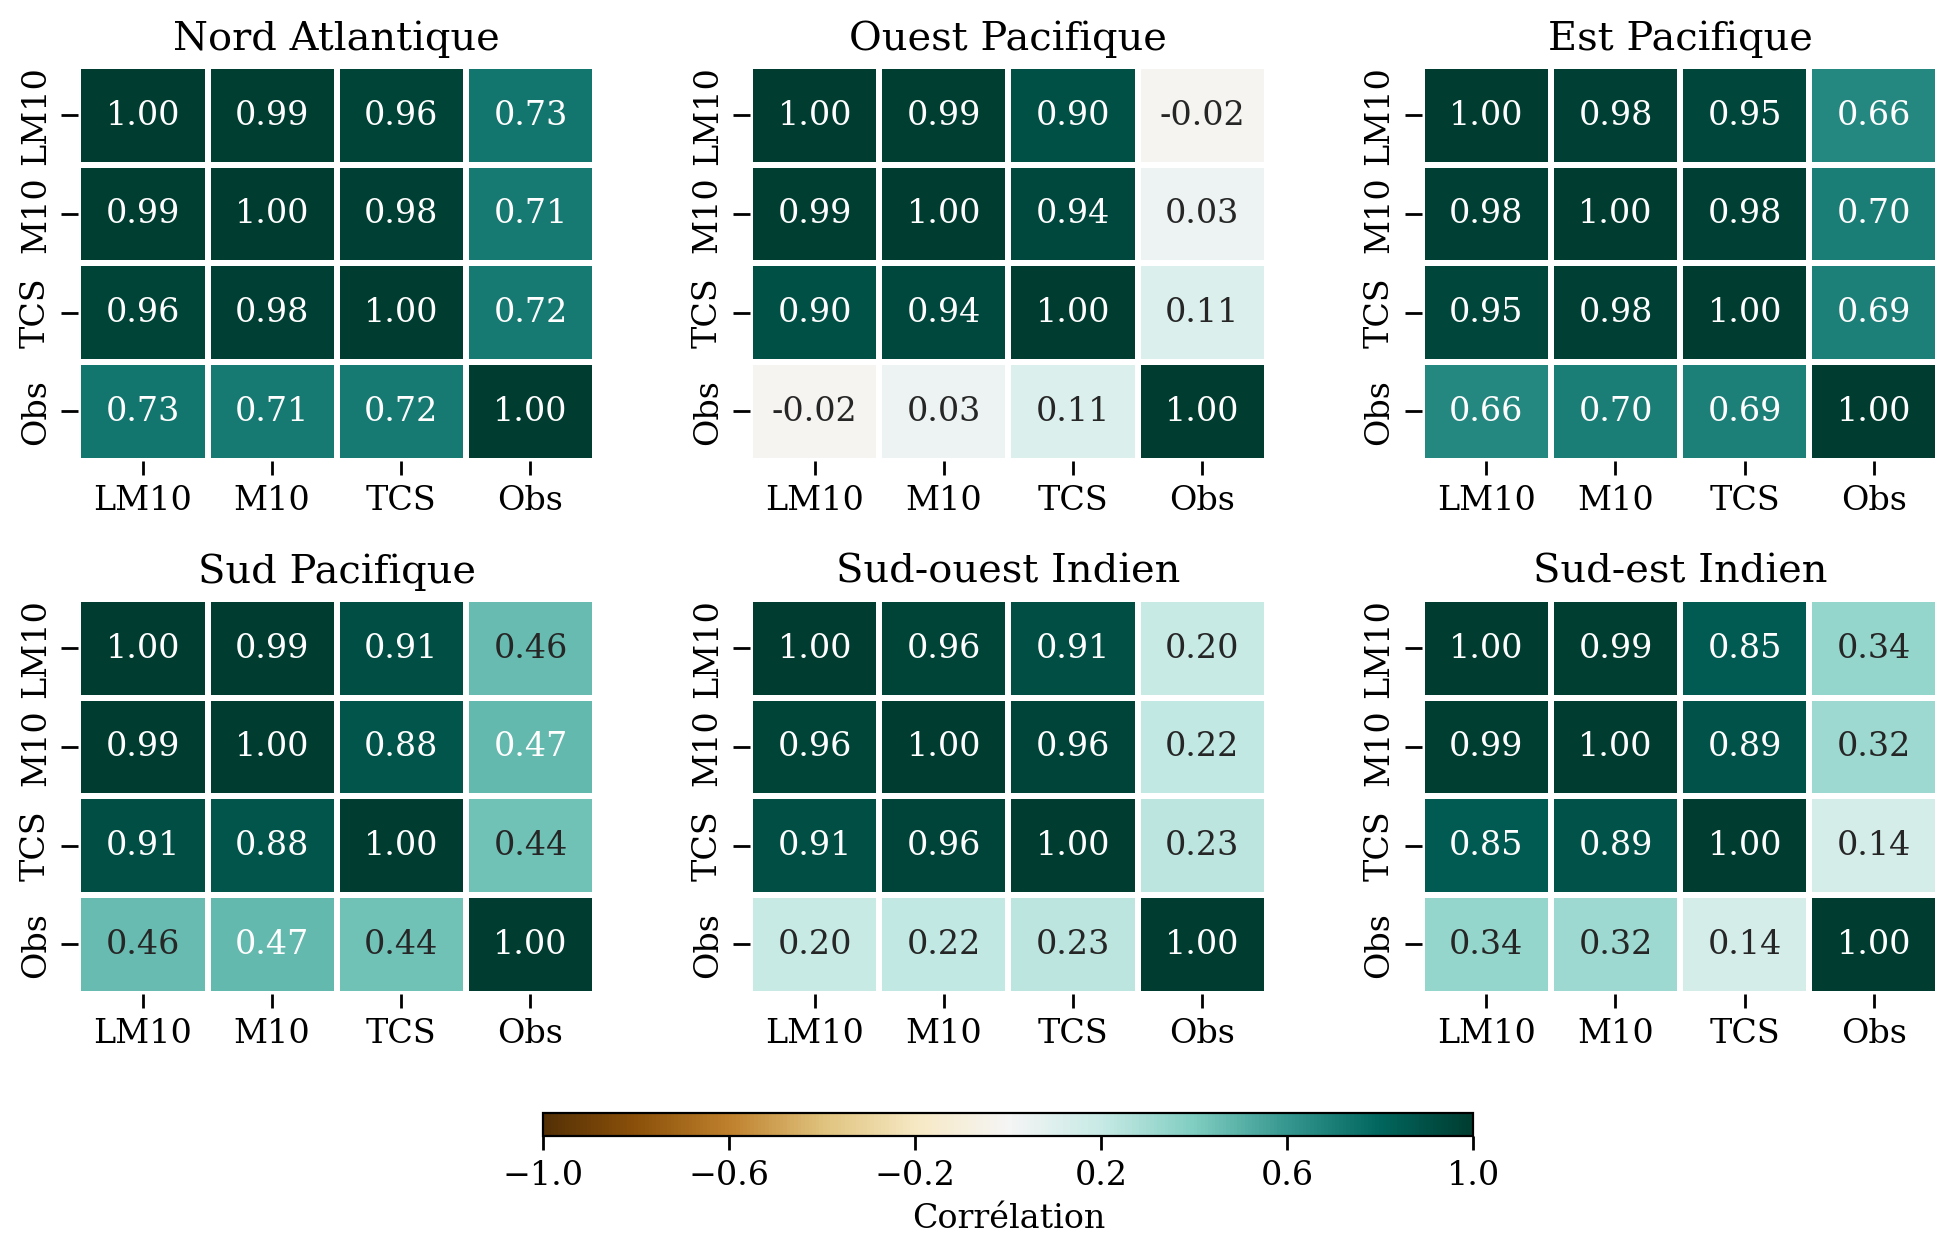
\includegraphics[width=\textwidth]{corr_lm10_m10_ibt.png}
    \caption{Matrices de corrélation entre les variations interannuelles du nombre de TC simulé par LM10, M10, TCS ainsi que la variabilité observée via IBTrACS
    (Obs) entre les saisons 1981 et 2019.}
    \label{fig:corr_lm10_m10_ibt}
\end{figure}

Comme attendu, LM10 présente des corrélations tout à fait comparables à M10, proches de \num{0.7} dans les bassins NAtl et EPac, \num{0.5} dans le SPac,
\num{0.2} dans le SIndW et \num{0.3} dans le SIndE. Seul le SIndE présente une corrélation améliorée pour LM10 et M10 avec IBTrACS, par rapport au TCS. Dans le
WPac, les corrélations pour LM10 et M10 sont dégradées (à \num{0}) par rapport au TCS, lequel n'est de toutes façons pas corrélé de manière significative avec
\num{0.11}. Par ailleurs, l'inhomogénéité du champ d'humidité dans ERA5 est peut-être responsable de ces mauvaises performances, si bien qu'on ne saurait trop
s'atarder sur l'interprétation des résultats dans ce bassin. À ces deux exceptions près, les trois indices présentent des corrélations proches les unes des
autres. Les bassins EPac et SIndW sont les deux seuls bassins pour lesquels LM10 présente une corrélation avec IBTrACS dégradée par rapport à M10 mais aussi par
rapport au TCS, bien que la différence soit à la deuxième décimale.

\subsection{Conclusion}

Dans cette section, les coefficients $b$ de la régression de Poisson ont été calculés à l'échelle des bassins océaniques en utilisant les prédicteurs de grande
échelle du TCS, aussi utilisés dans la \cref{sec:apport_res_temporel_spatial}. Les six régressions peuvent être vues comme un seul indice de cyclogénèse, défini
caractérisé par ses coefficients $b$, eux-même étant fonction de la région. Cet indice étant, outre sa dépendance régionale, construit selon la même
méthodologie que pour l'indice M10 de la \cref{sec:apport_res_temporel_spatial}, c'est à dire en appliquant la relation \ref{eq:poisson_reg} sur les champs
mensuels d'ERA5 interpolés sur une grille régulière de \ang{1}, ce nouvel indice régional est nommé LM10. Les résultats de la
\cref{sec:apport_res_temporel_spatial} indiquent que la construction d'un indice régional ne peut à priori pas améliroer la représentation de la variabilité
interannuelle, puisqu'il y est montré que les coefficients $b$ n'influent pas (ou peu) sur cette dernière, mais peut en revanche impacter la répartition
spatiale de l'activité cyclonique simulée dans chaque bassin. Par conséquent, un indice régional est à même d'apporter de l'information sur la sensibilité de la
fréquence d'occurrence des TC aux différentes variables de grande échelle à une échelle régionale, et peut de surcroît améliorer la répartition spatiale des TC
à cette même échelle.

Le nouvel indice de cyclogénèse LM10 met ainsi en évidence une sensibilité de la fréquence de cyclogénèses à l'environnement de grande échelle très variable
selon les régions (voir \cref{sec:lm10_coefficients}). Les coefficients associés à la vorticité absolue bornée $\eta$ ainsi qu'à la SST relative $T$ présente la
plus grande variabilité. Le bassin NAtl présente, de très loin, la plus grande sensibilité à la vorticité, avec un coefficient supérieur à \num{2}, tandis que
le bassin WPac présente au contraire une sensibilité moindre inférieure à \num{1} ---~les quatre autres bassins indiquant tous une sensibilité accrue par
rapport à M10. De la même manière, la sensibilité à la SST relative à l'échelle du bassin géographique est systématiquement plus grande que celle établie à
l'échelle globale avec M10, à l'exception du bassin NAtl, où cette dernière n'est que de \num{0.33}. En comparaison, les coefficients associés au cisaillement
vertical du vent et à l'humidité relative à \hPa{600} ne connaissent que peu de variations entre bassins océaniques, et demeurent relativement proches des
valeurs estimées pour M10.

Ces variations inter-régions dans les coefficients $b$ de l'indice LM10 se traduisent par une répartition spatiale modifiée de l'activité cyclonique simulée par
rapport à M10 (voir \cref{sec:lm10_effet_spatial}). Les bassins de l'hémisphère nord sont sensiblement plus impactés que ceux de l'hémisphère sud. Dans les
bassins EPac et NAtl, l'activité est principalement décalée vers le nord, tandis que dans le bassin WPac elle est au contraire décalée vers le sud. Dans les
trois bassins, ces changements aboutissent à une erreur quadratique moyenne évaluée entre IBTrACS et l'indice local diminuée par rapport à M10, indiquant une
meilleure ressemblance avec les observations (à l'exception notable du GoM dans le bassin NAtl). Les changements dans la répartition méridionale sont donc
inversés entre les bassins WPac d'une part et EPac et NAtl d'autre part. Or, il est désormais établit que la régression de Poisson vise avant tout à offrir une
bonne cohérence spatiale entre l'activité observée et l'activité simulée, plus qu'une bonne cohérence dans la variabilité temporelle (tout du moins à l'échelle
interannuelle), et que cette cohérence spatiale se fait par le biais des coefficients $b$ de la régression. Le bassin WPac étant le plus actif de tous, cela
indique que sa contribution dans une régression réalisée à l'échelle globale compte beaucoup. Il est alors permis de supposer que les différences entre bassins
de la répartition méridionale de l'activité cyclonique dans l'hémisphère nord est à l'origine de la mauvaise distribution méridionale simulée dans cet
hémisphère pour les indices construits à l'échelle globale (voir aussi \cref{fig:tcs_cygp_gpi_zonal,fig:my_fit_meridional}). Les indices construits à l'échelle
régionale permettent par conséquent de corriger ces biais et d'offrir localement une meilleure ressemblance avec l'activité observée.

%Dans les
%bassins EPac et WPac, la répartition spatiale de l'activité cyclonique avec LM10 est distinctement plus proche de l'activité observée dans IBTrACS. En
%particulier, l'activité est focalisée le long de la côte du Mexique dans le bassin EPac, autour de \ang{90}W. Ce résultat est atteint en augmentant la
%sensibilité à la SST relative (à sa valeur la plus haute dans cette région) ainsi qu'en augmentant plus modestement la sensibilité à la vortcité, par rapport à
%M10. Dans le bassin WPac, l'activité cyclonique inférée par LM10 est au contraire déportée vers l'équateur, par le biais notamment d'une baisse importante de la
%sensibilité à la vorticité. Rappelons en effet que la sensibilité à la vorticité a pour conséquence notable de piloter la répartition méridionale de l'activité
%cyclonique, comme montré dans la \cref{sec:apport_res_temporel_spatial}. Dans les deux bassins, l'erreur quadratique moyenne entre IBTrACS et l'activité simulée
%est réduite avec LM10, indiquant une meilleure ressemblance avec la densité de cyclogénèses observées. Dans le bassin NAtl, l'activité est déportée vers le nord
%en faveur de la MDR, se rapprochant ainsi des observations, mais l'activité est réduite dans le GoM, ce qui constitue une dégradation par rapport à M10, qui
%dans ce sous-domaine est plus proche d'IBTrACS. À l'échelle du bassin, l'erreur quadratique moyenne est tout de même améliorée.


%\section{Exploration du potentiel prédictif d'un indice à l'échelle saisonnière}
%
%\subsection{Choix du pas d'agrégation temporelle : Mensuel versus saisonnier}
%
%\subsection{Effet de la résolution spatiale et temporelle}\label{sec:resolution_spatiale_temporelle}
%
%\subsection{Activité observée versus modèle ARPEGE}
%
%\subsection{Scores de performances sur la variabilité inter-annuelle}


%--------------------------------------
\section{Synthèse}

Dans ce chapitre, plusieurs indices de cyclogénèse ont été appliqués à la réanalyse ERA5 du CEPMMT, au pas de temps mensuel et à la résolution spatiale de
\ang{1}. Dans une première partie, les indices les plus communément utilisés dans la littérature ont étés présentés. Ces derniers peuvent être distingués entre
ceux dont la construction est partiellement empirique ---~notamment dans le choix des pondérations appliquées à chacun des prédicteurs de grande échelle~--- ou
bien si l'indice est construit comme une régression statistique. Trois indices sont retenus : Le GPI \parencite{emanuel_tropical_2004}, le CYGP
\parencite{royer_gcm_1998} et le TCS \parencite{tippett_poisson_2011}. Ces indices sont évalués sur ERA5, puis comparés entre eux ainsi qu'avec les observations
issues de la base de données IBTrACS entre \num{1981} et \num{2019}. Cette comparaison identifie les mêmes atouts et limitations des indices que les travaux de
\textcite{menkes_comparison_2012}, lesquels appliquent ces trois mêmes indices à quatre réanalyses entre \num{1979} et \num{2001}. En particulier, tous les
indices considérés surestiment l'activité dans l'hémisphère sud et la sous-estiment dans l'hémisphère nord. De plus, la distribution méridionale de l'activité
annuelle moyenne est excellente dans l'hémisphère sud, tandis qu'aucun indice ne la simule correctement dans l'hémisphère nord, le TCS étant cependant le plus
proche sur les deux tableaux. Tous les indices présentent par ailleurs une activité simulée trop importante dans la vicinité immédiate de l'équateur. Dans
l'ensemble, le cycle annuel de l'activité cyclonique dans chacun des bassins oćeaniques est correctement reproduit, aussi bien dans leur saisonnalité que dans
l'amplitude. Une exception notable concerne le CYGP qui peine à simuler la bi-saisonnalité du bassin NInd, et qui sous-estime fortement l'activité dans le
bassin NAtl. Le TCS se distingue à nouveau des deux autres en étant l'indice minimisant au mieux l'activité en dehors de la saison cyclonique, à l'exception des
bassins SPac et NInd. Les indices parviennent donc à simuler la climatologie de l'activité observée avec une grande fidélité, mais sont nettement moins aptes à
simuler les variations interannuelles. Seules les régions EPac et NAtl présentent une bonne corrélation entre la variabilité simulée et celle observée. Dans le
bassin EPac, les series temporelles sont d'ailleurs remarquablement proches, les indices simulant aussi bien la variabilité que l'amplitude observée.

Dans une seconde partie, l'apport de la résolution spatiale et temporelle a été évaluée pour un indice construit selon la même méthodologie que le TCS. Ce
dernier, dont les coefficients sont le résultat d'une régression de Poisson entre l'environnement de grande échelle et l'activité observée, présente en effet
l'intérêt d'être facilement reproductible, et se prête donc mieux aux expérimentations. L'effet de la résolution spatiale accrue dans la régression (passant de
\ang{2.5} à \ang{1}), de même que l'introduction de variabilité temporelle à plus haute fréquence (champs mensuels contre les moyennes climatologiques), sur les
coefficients de la régression ont été étudiés, de même que l'effet des changements de coefficients sur l'indice en résultant. La modification des coefficients
$b$ de la régression se traduit par une modification de la répartition spatiale de l'activité cyclonique inférée par l'indice. Il est montré que l'effet est
similaire aussi bien pour la résolution spatiale accrue que l'usage de champs mensuels climatologiques, mais que l'effet de la variabilité temporelle est
dominant (voir \cref{sec:apport_resultat}). Spécifiquement, la sensibilité accrue à la vorticité absolue, résultant de l'usage de champs mensuels, permet la
correction du biais équatorial du TCS. Il est toutefois soulevé que les coefficients de la régression ne sont pas particulièrement robustes, notamment car la
période temporelle utilisée pour faire la régression semble jouer un rôle important dans les valeurs prises par les coefficients. Une dérive des coefficients
par rapport à ceux du TCS est en effet notée lorsque la période de référence s'éloigne de celle utilisée par \textcite{tippett_poisson_2011}. Cette dérive
ramène à la problématique de la (non-)stationnarité dans le temps des relations proposées par les différents indices de cyclogénèse, et donc de leur validité
pour l'étude du climat futur. Cependant, les moyens manquent pour confirmer ou non cette tendance.

En dépit des variations importantes dans les coefficients $b$ des différentes régressions essayées dans le cadre de ce travail, la variabilité interannuelle
inférée par les indices nouvellement construits ne s'en retrouve que très peu affectée. La variabilité interannuelle des quatre indices définis dans la
\cref{sec:apport_res_temporel_spatial} apparaissent quasiment indiscernables les unes des autres, et les différences entre celles-ci et la variabilité
interannuelle du TCS sont à peine plus prononcées. Il en résulte donc naturellement que la corrélation entre la variabilité interannuelle et les observations
n'est pas améliorée. Puisque les coefficients n'impactent que marginalement la variabilité temporelle des indices de cyclogénèse, il en découle que cette
dernière doit être contrôlée par le choix des prédicteurs utilisés. Mais malgré l'absence d'amélioration, le diagnostique introduit dans la
\cref{sec:diagnostique_rang}, basé sur la mesure de la distribution des rangs des valeurs prises par l'indice aux points de grille correspondant aux
cyclogénèses observées, montre que la détermination de coefficients mieux adaptés à un jeu de donné cible possède tout de même un intérét. Il est en effet
montré que les indices nouvelles construits sont plus actifs que le TCS en lieu et date d'une cyclogénèse observée, y compris pour l'indice visant à reproduire
le plus fidèlement possible ce dernier.

Enfin, une troisième partie de ce chapitre (voir \cref{sec:indice_regional}) a été consacrée à la définition d'un indice de cyclogénèse régional. Il s'agit en
réalité de plusieurs indices, construits par régression de Poisson à l'échelle des bassins océaniques, qui peut être utilisé comme un indice pseudo-global, dont
les coefficients sont fonction du bassin. Comme vu précédemment, une telle approche ne peut améliorer la variabilité interannuelle, mais il est montré que la
construction d'indices locaux peut apporter de l'information utile sur la sensibilité de la fréquence d'occurrence des TC aux variables de grande échelle à
l'échelle d'un bassin océanique. L'indice régional impacte sensiblement la répartition géographique de l'activité cyclonique simulée dans l'hémisphère nord,
tandis que l'effet est minime dans l'hémisphère sud. La régression menée à l'échelle du bassin offre alors une amélioration de la ressemblance entre l'activité
simulée et l'activité observée (voir aussi \cref{sec:lm10_effet_spatial}). Il est notamment noté que l'indice régional déporte l'activité vers l'équateur dans
le bassin WPac, tandis qu'il la décale vers le nord dans les bassins NAtl et EPac. Ces changements réduisent dans tous les cas l'erreur quadratique moyenne avec
IBTrACS. Il est alors suggéré que la disparité dans la répartition en latitude de l'activité cyclonique puisse être à l'origine de la difficulté rencontrée par
tous les indices de cyclogénèse construits à l'échelle globale à simuler une distribution méridionale réaliste.


\end{document}
